\PassOptionsToPackage{table}{xcolor}
\let\brlBibliographystyle\bibliographystyle
\renewcommand{\bibliographystyle}[1]{\brlBibliographystyle{brl-mathphys-ay}}
\documentclass[pdflatex,iicol,sn-mathphys-ay]{sn-jnl}
\let\bibliographystyle\brlBibliographystyle

\usepackage{graphicx}
\usepackage{amsmath}
\usepackage{amssymb}
\usepackage{comment}
\usepackage{algpseudocode}
\usepackage[linesnumbered,ruled,vlined]{algorithm2e}
\usepackage{multirow}
\usepackage[most]{tcolorbox}
\usepackage{float}
\usepackage[normalem]{ulem}
\usepackage{xcolor}
\usepackage{subcaption}
\usepackage{stmaryrd}
\usepackage{tabularx}
\usepackage{booktabs}
\usepackage{diagbox}
\usepackage{makecell}
\usepackage{tikz}
\usepackage{array}
\usepackage{setspace}
\usepackage{pifont}

\newcommand{\cmark}{\ding{51}}
\newcommand{\xmark}{\ding{55}}
\newcommand{\omark}{\ding{108}}

\definecolor{darkblue}{rgb}{0.15,0.15,0.55}
\definecolor{lightgrey}{rgb}{0.75,0.75,0.75}
\newcommand{\qedm}{\hfill $\square$}
\DeclareUnicodeCharacter{25B3}{\ensuremath{\triangle}}
\newcommand\ny[1]{{\color{magenta}{#1}}}
\newcommand\sj[1]{{\color{violet}{#1}}}
\newcommand\sh[1]{{\color{orange}{#1}}}
\newcommand\gy[1]{{\color{purple}{#1}}}
\newcommand\cp[1]{{\color{blue}{#1}}}
\newcommand\jh[1]{{\color{green}{#1}}}

\hyphenation{op-tical net-works semi-conduc-tor}
\raggedbottom

\begin{document}

% \title[When and What to Ask External Experts during Robot Task Planning under State Uncertainty]{When and What to Ask External Experts during Robot Task Planning under State Uncertainty}

\title{When and What to Query in Robot Task Planning under Partial Observability}

\author[1]{\fnm{Changmin} \sur{Park}}\email{cmp9877@gmail.com}
\equalcont{These authors contributed equally to this work.}

\author[1]{\fnm{Seongah} \sur{Park}}\email{ppseongah@gmail.com}
\equalcont{These authors contributed equally to this work.}

\author[1]{\fnm{Nayoung} \sur{Kim}}\email{nayoungkim0826@gmail.com}
\author[1]{\fnm{Sungjin} \sur{Park}}\email{sungjin.park@sogang.ac.kr}
\author[1]{\fnm{Gayoung} \sur{Ryu}}\email{gyryu.sg@gmail.com}
\author[1]{\fnm{Geonyeong} \sur{Ko}}\email{2567bear@naver.com}
\author*[1]{\fnm{Junho} \sur{Lee}}\email{junho.lee@sogang.ac.kr}
\author*[1,2]{\fnm{Changjoo} \sur{Nam}}\email{cjnam@sogang.ac.kr}

\affil*[1]{\orgname{Sogang University},
  \orgaddress{\city{Seoul}, \country{Republic of Korea}}}
\affil[2]{\orgname{Vertical Labs},
  \orgaddress{\city{Seoul}, \country{Republic of Korea}}}


\abstract{In this paper, we present a method for deciding when a robot should request external information and what it should ask during task planning. A robot with incomplete information may fail to determine the current state of the world, which can lead to task failure. However, resolving all uncertainty through external queries would incur unnecessary costs. Therefore, a robot must determine both when to query and what information to request. To solve this problem, we construct a weighted belief over possible current states. We use belief uncertainty to decide when to query and select the query expected to reduce uncertainty the most. After receiving an answer from an external agent, we update the belief and continue task planning. 
% We evaluate the framework on two robotic domains against existing proactive querying systems during task planning. In simulation with correct responses, our method achieves success rates of $100.00\%$ and $97.50\%$ versus $76.00\%$ and $56.00\%$ for the best baseline. The success advantage holds with vision language model and human feedback on physical robots. Ablation experiments show that our query timing maintains high success, while our query selection reduces query counts under the same timing criterion.
We evaluate the framework in two robotic domains against existing proactive querying systems during task planning. Our system achieves higher task success rates than the baselines in simulation and in physical robot trials with vision language model or human feedback. Ablation results show that our timing method improves task success and our selection method reduces the number of queries.

}

\keywords{Planning under uncertainty, online symbolic planning, robotic systems}

\maketitle

\section{Introduction}~\label{intro}
% Robots operating in real-world environments often have incomplete or unreliable information about the current state due to perception errors~\citep{kaipa2016addressing}, execution failures~\citep{kaelbling1998planning}, and unexpected environmental changes~\citep{kurniawati2016online}. If such uncertainty is not resolved, the robot may make incorrect decisions and fail the task. In practice, relying on an external agent to recognize the need for assistance requires continuous monitoring of robot execution. The robot must therefore be able to detect uncertainty and initiate queries to obtain additional information before proceeding~\citep{dragan2013legibility, goodrich2008human}. However, frequent queries can incur substantial costs in time and workload~\citep{chen2014human}. The robot must therefore determine \textit{when} to request external feedback and 
Robots often encounter uncertainty during task planning due to perception errors~\citep{kaipa2016addressing} and action failures~\citep{kaelbling1998planning}. For example, a robot may be uncertain whether a tomato is ripe or whether a pick action succeeded. The robot can proactively ask an external agent to provide missing information or select the next action to reduce the need for continuous monitoring by the external agent. However, too few queries can leave uncertainty unresolved and lead to task failure, whereas frequent queries increase interaction costs, such as response latency, token use for a vision language model (VLM), and human workload. A further challenge is that simply increasing the number of queries does not necessarily improve task success. The robot may still fail if queries come late or do not resolve the uncertainty. The robot must therefore determine \textit{when} to ask for help and \textit{what} information to request for task success while limiting the number of queries.

% Recent uncertainty-aware systems selectively request external feedback during task execution. Existing approaches commonly trigger queries based on prediction confidence, including conformal prediction~\citep{ren2023robots, liang2024introspective, mullen2025lbap}, or on the expected effect of a query on task reward~\citep{burks2021collaborative, anand2025adaptive}. However, a confident action prediction does not ensure that the underlying state estimate is correct. Under reward-based criteria, the robot may also execute an action without querying even when state uncertainty remains. Both approaches can therefore miss opportunities to verify the state information needed for successful execution, leading to task failure. We use state uncertainty to determine when verification is needed and expected uncertainty reduction to select what to ask.
% Existing system-initiative querying methods often use action prediction confidence or expected return to guide querying decisions. For example, KnowNo uses conformal prediction sets to determine when to request an action choice~\citep{ren2023robots}, while IntroPlan combines conformal prediction with retrieved reasoning examples for candidate evaluation~\citep{liang2024introspective}. Yet both methods may proceed without querying if incorrect perception produces a confident action prediction. Even when assistance is requested, the candidate set may not include a correct action. POMDP-based approaches~\citep{burks2021collaborative,burks2023harps} model candidate queries as planning actions and determine when and what to query by maximizing expected cumulative reward. However, maximizing cumulative rewards for task performance does not necessarily yield efficient querying, because asking fewer questions can increase the risk of failure, while asking more does not always improve task success.
Existing methods often use confidence in predicted actions or expected reward return to decide when and what to query. Methods based on conformal prediction (CP) query an external agent if multiple candidate actions remain~\citep{ren2023robots,liang2024introspective}. However, a single candidate does not ensure a correct state estimate, and the prediction set may exclude the correct action. Approaches based on a partially observable Markov decision process (POMDP) model queries as planning actions~\citep{burks2021collaborative,burks2023harps} and select them according to expected cumulative reward. However, neither approach explicitly determines whether the current state is sufficiently certain. Consequently, the robot may plan with insufficient state information or ask unnecessary queries.


% In this paper, we present a belief-based method for deciding when to request external feedback and what to ask. We formulate task planning as a POMDP~\citep{kaelbling1998planning} and maintain a knowledge base containing symbolic facts and STRIPS-style action models~\citep{davis1993knowledge,fikes1971strips}. After each action, the robot uses these facts and action models to generate reachable states and constructs a weighted belief using the resulting observation. If belief confidence falls below a threshold, the robot asks an external agent to verify the state fact with the greatest expected entropy reduction. The robot updates the belief after each response and continues querying until the confidence reaches the threshold. The robot then updates the facts in the knowledge base and resumes planning and execution.
% In this paper, we present a method that uses uncertainty about the current symbolic state to determine when to query and what to ask. We formulate task planning as a POMDP~\citep{kaelbling1998planning} and use symbolic facts and action models~\citep{davis1993knowledge,fikes1971strips} to construct a weighted belief over reachable states. To determine when to query, the robot computes belief confidence from normalized entropy, which decreases as probability concentrates on a single state. The robot queries an external agent if belief confidence falls below a threshold. To determine what to query, the robot selects the state fact with the greatest expected reduction in belief entropy to reduce the number of queries needed to reach the confidence threshold. Each response provides evidence for updating the belief. Once confidence reaches the threshold, the robot updates the knowledge base with the maximum a posteriori state estimate and resumes planning and execution.

In this paper, we present a method that uses uncertainty about the current symbolic state to determine when to query and what to ask. We formulate task planning as a POMDP~\citep{kaelbling1998planning} and use symbolic facts and action models~\citep{davis1993knowledge,fikes1971strips} to construct a weighted belief over reachable states. To determine when to query, the robot computes belief confidence from normalized entropy, which decreases as probability concentrates on a single state. The robot queries an external agent if the confidence falls below a threshold. To determine what to query, the robot selects the fact with the greatest expected reduction in belief entropy. Each response rules out states that conflict with the answer. We use the maximum a posteriori (MAP) state to update the knowledge base and resume planning. We construct the next frontier from the MAP state and the next action.



% We evaluate the method in two robotic domains. In simulation with correct oracle responses, we compare our method with conformal prediction based and reward-based strategies and analyze the effects of query timing and query selection. We then conduct physical robot experiments with feedback from a vision-language model (VLM) and human participants, comparing our method with the conformal prediction based method. Interviews with the five participants provide qualitative insights into their experiences with both methods. Our method achieves higher task success rates than all evaluated baselines in simulation and than the selected baseline with VLM and human feedback on physical robots. Ablation results indicate that query timing primarily affects task success, while query selection reduces the number of queries required.

% We evaluate our method on two robotic tasks in partially observable environments with sensing errors. In simulations with an oracle agent, we compare our method against two query strategies based on conformal prediction and expected task reward, respectively. We then conduct physical robot experiments using a VLM and human participants as external agents to compare our method with a baseline based on conformal prediction. Our method achieves the highest success rates in both simulation and physical robot experiments with VLM and human feedback. Ablation experiments show that query timing mainly affects task success, while our query selection method reduces the number of queries with the same timing criterion. We also vary the confidence threshold to examine the trade-off between task success and query count. Finally, interviews with all five participants help explain the differences in task performance between the two methods.
We evaluate our method on two robotic tasks in partially observable environments with sensing errors. In simulations with an oracle agent, we first compare our system against existing proactive querying systems based on CP and expected task reward. We then conduct physical robot experiments with VLM and human feedback to compare our method with a CP baseline. Our method achieves the highest success rates among the evaluated systems across all baseline experiments. We then conduct ablation experiments with the same POMCP planner to distinguish the effects of query timing and selection on task success and query count. Ablation experiments show that query timing based on confidence maintains high success across selection strategies, while query selection based on expected entropy reduction reduces the number of queries under the same timing criterion. We also vary the confidence threshold to examine the tradeoff between task success and query count. Finally, interviews with all five participants help explain the differences in task performance between the two methods.

% The contributions of this work are as follows:
% \begin{itemize}
% \item We determine when to query based on uncertainty in the current belief and show that query timing has a substantial effect on task success.
% \item We choose what to query using expected entropy reduction and show that query selection reduces query counts compared to the baselines.
% \item We evaluate the proposed method in simulation and on physical robots with VLM and human feedback, demonstrating higher task success than the evaluated baselines.
% \end{itemize}
Our contributions are as follows:
\begin{itemize}
\item We determine when to query from belief uncertainty to improve task success.
\item We select what to query by expected entropy reduction, reducing query counts under a fixed timing criterion.
\item We demonstrate higher task success than the evaluated baselines in simulation and on physical robots with VLM and human feedback.
\end{itemize}
\section{Related Work}~\label{related}
We review prior work on representing state uncertainty in symbolic planning and on determining when and what to query under uncertainty.

\subsection{State Uncertainty in Symbolic Planning}~\label{rel:state_uncertainty}
We consider uncertainty about which facts hold in the current task state. Perception errors and uncertain action outcomes can leave several states consistent with the available observations. Symbolic planning represents each state as a set of facts and describes actions through preconditions and effects~\citep{fikes1971strips,mcdermott1998pddl}. Classical planning assumes a known current state and deterministic action outcomes. Probabilistic PDDL (PPDDL) extends this representation with probabilistic action effects and rewards~\citep{younes2004ppddl1}. The Relational Dynamic Influence Diagram Language (RDDL) describes probabilistic state transitions and observation models for partially observable domains~\citep{sanner2010rddl}. POMDPs represent uncertainty over possible current states through a belief and use anticipated observations in action selection~\citep{kaelbling1998planning}. Within this research direction,~\citet{zhang2015corpp} use commonsense reasoning to construct prior beliefs for POMDP planning, and \citet{sanner2010symbolic} use first order structure for symbolic dynamic programming. We use symbolic facts and action models to construct a weighted belief over reachable successor states during execution.


Maintaining an exact belief over all possible states is often computationally intractable in large state spaces. Particle representations approximate the belief with a finite set of sampled states~\citep{thrun2005probabilistic}. Online POMDP methods reduce computation by planning from the current belief without computing a policy over the entire belief space~\citep{ross2008online}. Partially Observable Monte Carlo Planning (POMCP) combines Monte Carlo belief updates with Monte Carlo tree search for online action selection~\citep{silver2010monte}. The work of~\citet{xiao2019objectsearch} extends POMCP to target object search in clutter under perception and manipulation uncertainty. 
% However, prior work on online POMDP planning focuses on action selection under state uncertainty without explicitly querying an external agent. We propose a method that integrates action selection with querying.
We ask an external agent to verify facts that distinguish the candidate states. As answers rule out inconsistent states, belief weight can concentrate on one state even while other states remain plausible. We therefore use the most probable remaining state to resume symbolic planning.


\subsection{Query Timing and Selection under Uncertainty}~\label{rel:selective_querying}
Existing methods determine query timing from uncertainty estimates, human trust, or ambiguity among candidate actions. Some methods use uncertainty in task return~\citep{singi2023hula} or implicit uncertainty estimates learned from a visual navigation policy~\citep{igbinedion2024learning}. \citet{mangalindan2025seek} model human trust in the robot as a latent POMDP state and use the trust model to select assistance requests for team performance. Online conformal prediction guides requests for expert feedback in interactive imitation learning~\citep{zhao2025conformalized}. KnowNo requests an action choice if its conformal prediction set contains multiple candidates~\citep{ren2023robots}, and IntroPlan combines conformal prediction with retrieved introspective reasoning examples~\citep{liang2024introspective}. Query timing in KnowNo and IntroPlan depends on ambiguity among candidate actions, without an explicit belief over symbolic task states.


POMDP-based methods model information requests as planning actions to determine query timing and selection through expected cumulative reward~\citep{armstrongcrews2007oracular,burks2021collaborative,burks2023harps}. Oracular POMDPs consider an oracle that reveals the exact state at a fixed cost~\citep{armstrongcrews2007oracular}. Human assisted semantic sensing incorporates human observations into the belief and selects queries through the planning objective~\citep{burks2021collaborative,burks2023harps}. Therefore, existing methods determine when and what to query based on query costs and expected rewards. We use belief confidence to decide when to query.



Query selection depends on the information needed for the task. \citet{kaipa2016addressing} use human input to resolve perception uncertainty in bin-picking. \citet{deits2013clarifying} select questions that reduce entropy in the mapping between natural language commands and entities in the environment. \citet{anand2025adaptive} use information gain to choose feedback formats at critical states for penalty function learning, considering feedback cost and availability. In contrast, our method selects the state fact that maximizes the expected reduction in belief entropy through a query to an external agent.


\section{Preliminaries}~\label{preliminaries}
% The objective of planning is to find a transition sequence that transforms the initial state into a goal state. 
A symbolic planning problem is a tuple $\mathcal{P}=\langle\mathcal{F},\mathcal{A},s_0,\mathcal{G}\rangle$, with a finite set of facts $\mathcal{F}$, actions $\mathcal{A}$, initial state $s_0\subseteq\mathcal{F}$, and goal condition $\mathcal{G}\subseteq\mathcal{F}$. Each state is a subset of $\mathcal{F}$. An action $a\in\mathcal{A}$ has preconditions $\mathrm{pre}(a)$, add effects $\mathrm{add}(a)$, and delete effects $\mathrm{del}(a)$.
% We can say that $a$ is applicable in $s$ if and only if $\mathrm{pre}(a) \subseteq s$, denoted as $a \llbracket s \rrbracket$. 
Here, $a$ is applicable in $s$ when $\mathrm{pre}(a)\subseteq s$, denoted by $a\llbracket s\rrbracket$, and produces $s^\prime=(s\setminus\mathrm{del}(a))\cup\mathrm{add}(a)$. A plan $\pi=(a_1,\ldots,a_T)$ applies actions from $s_0$ to reach a state $s_T$ satisfying $\mathcal{G}\subseteq s_T$.

A POMDP is a tuple $\langle\mathcal{S},\mathcal{A},T,R,\Omega,O,\gamma\rangle$, where $\mathcal{S}$, $\mathcal{A}$, and $\Omega$ are the state, action, and observation spaces. The models $T(s^\prime\mid s,a)$ and $O(o\mid s^\prime,a)$ give transition and observation probabilities, $R(s,a)$ is the immediate reward, and $\gamma\in(0,1]$ discounts future rewards. A belief $b$ is a probability distribution over states. After action $a$ and observation $o$, the Bayes filter updates it as
\[
b^\prime(s^\prime) = \eta \, O(o \mid s^\prime,a) \sum_{s \in \mathcal{S}} T(s^\prime \mid s,a) \, b(s),
\]
where $\eta$ normalizes the distribution. A policy maps beliefs to actions to maximize expected discounted reward $\mathbb{E}[\sum_{t=0}^{\infty}\gamma^t r_t]$.

Partially Observable Monte Carlo Planning (POMCP) searches over action-observation histories $h=\langle a_1o_1\cdots a_to_t\rangle$ using Monte Carlo tree search and a particle belief $B(h)$ at each history. It selects actions using the upper confidence bound (UCB) rule
\begin{equation}~\label{eq:ucb}
a^* = \arg\max_a \left( V(ha) + c \sqrt{\frac{\log N(h)}{N(ha)}} \right),
\end{equation}
where $V(ha)$ is the estimated action value, $N(h)$ and $N(ha)$ are visit counts, and $c$ controls exploration. Simulations sample transitions, observations, and rewards from a generative model. The discounted return $R=r+\gamma R^\prime$ updates the value by $V(ha)\leftarrow V(ha)+(R-V(ha))/N(ha)$. States sampled at each history form $B(h)$, approximating the posterior without explicit Bayes updates in the search tree.

\SetKwProg{Proc}{procedure}{}{}
\SetKwFunction{Search}{SEARCH}
\SetKwFunction{SampleParticle}{SAMPLE-PARTICLE}
\SetKwFunction{Simulate}{SIMULATE}
\SetKwFunction{Timeout}{TIMEOUT}
\SetKwFunction{Maxstep}{MAX-STEP}
\SetKwFunction{SearchBest}{SEARCH-BEST}
\SetKwFunction{UCB}{UCB}
\SetKwFunction{Rollout}{ROLLOUT}
\SetKwFunction{UpdateBelief}{UPDATE}
\SetKwFunction{ComputeConfidence}{CONF}
\SetKwFunction{SelectBestHypothesis}{SELECT-FACT}
\SetKwFunction{QuerySource}{QUERY}
\SetKwFunction{FilterBelief}{FILTER}



\begin{figure*}[t!]
\captionsetup{skip=0pt}
\centering
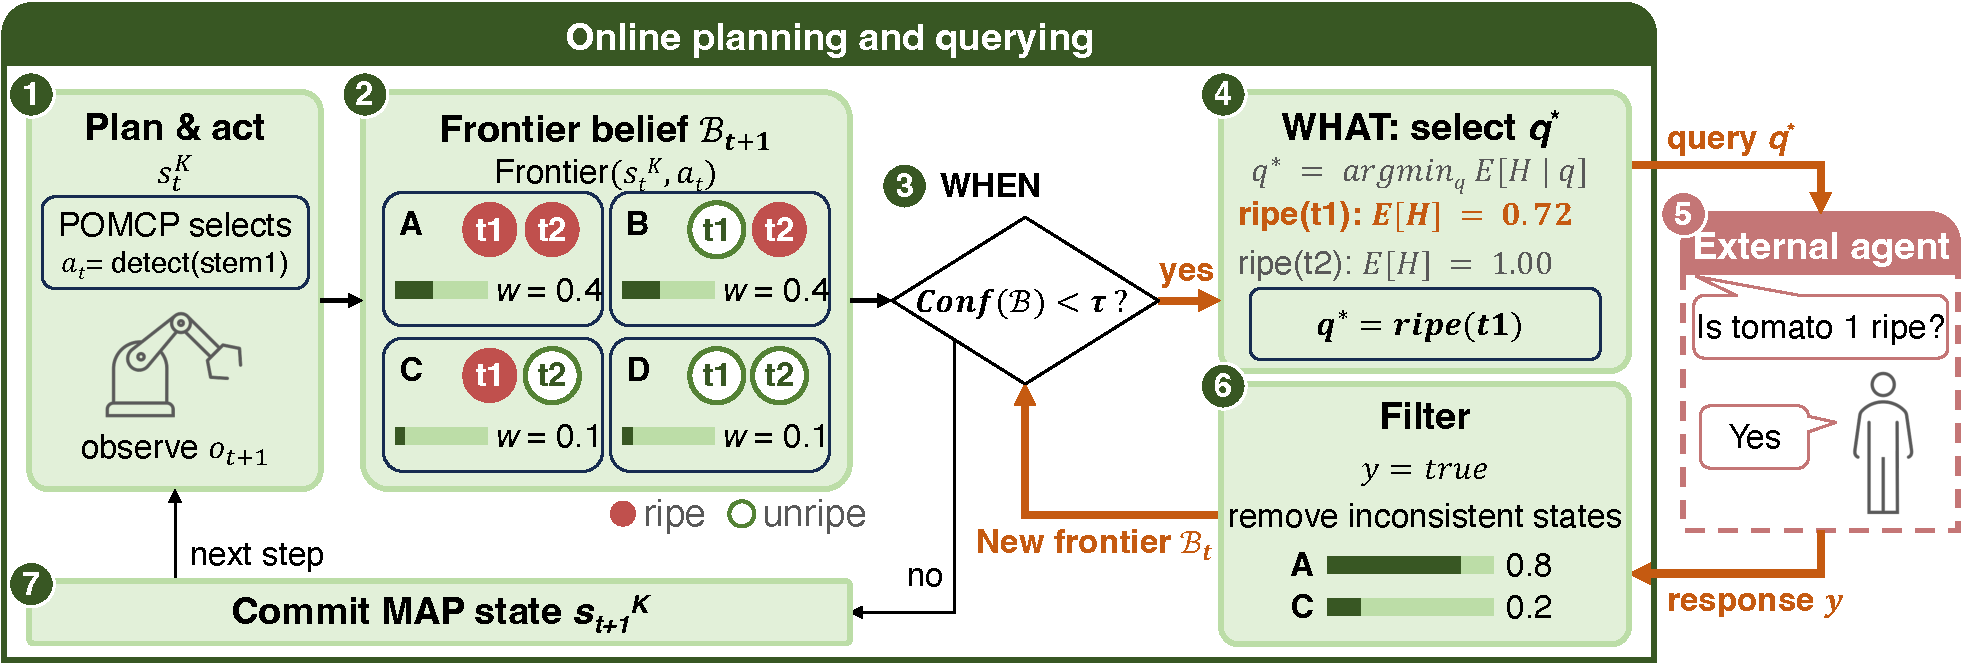
\includegraphics[width=0.995\linewidth]{figures/fig_method.pdf}
\caption{Online planning and querying. After $a_t$ and $o_{t+1}$, the robot constructs a frontier belief over candidate states. If belief confidence falls below $\tau$, robot queries $q^*$ that minimizes expected posterior entropy. The Boolean response $y\in\{\texttt{true},\texttt{false}\}$ filters inconsistent states, and the remaining weights are normalized. Querying repeats until the confidence threshold is met. The robot then commits the maximum a posteriori (MAP) state to the knowledge base and proceeds to the next planning step.}
\label{fig:planning_and_query}
\end{figure*}


\section{Method}~\label{method:method}
We first describe the online planning and querying procedure, which uses state uncertainty to determine when and what to query. We then present the system implementation for robot execution.
% \vspace{-25pt}
\subsection{Planning and Querying}~\label{method:overview}\label{method:planning}\label{method:PM}
We use a knowledge state $s_t^{K}$ for symbolic planning. For online action selection, we employ POMCP~\citep{silver2010monte}, restricting tree expansion and rollout to $a\llbracket s_t^{K}\rrbracket$. Therefore, at each step, the planner selects $a_t\llbracket s_t^{K}\rrbracket$. Following $a_t$ and $o_{t+1}$, we construct a weighted belief $\mathcal{B}_{t+1}$ by sampling from the reachable state frontier defined by $(s_t^{K},a_t)$. This restricts belief construction to symbolically valid successors while capturing uncertainty in the action outcome.


% \begin{figure*}[t]
% \captionsetup{skip=0pt}
% \centering
% 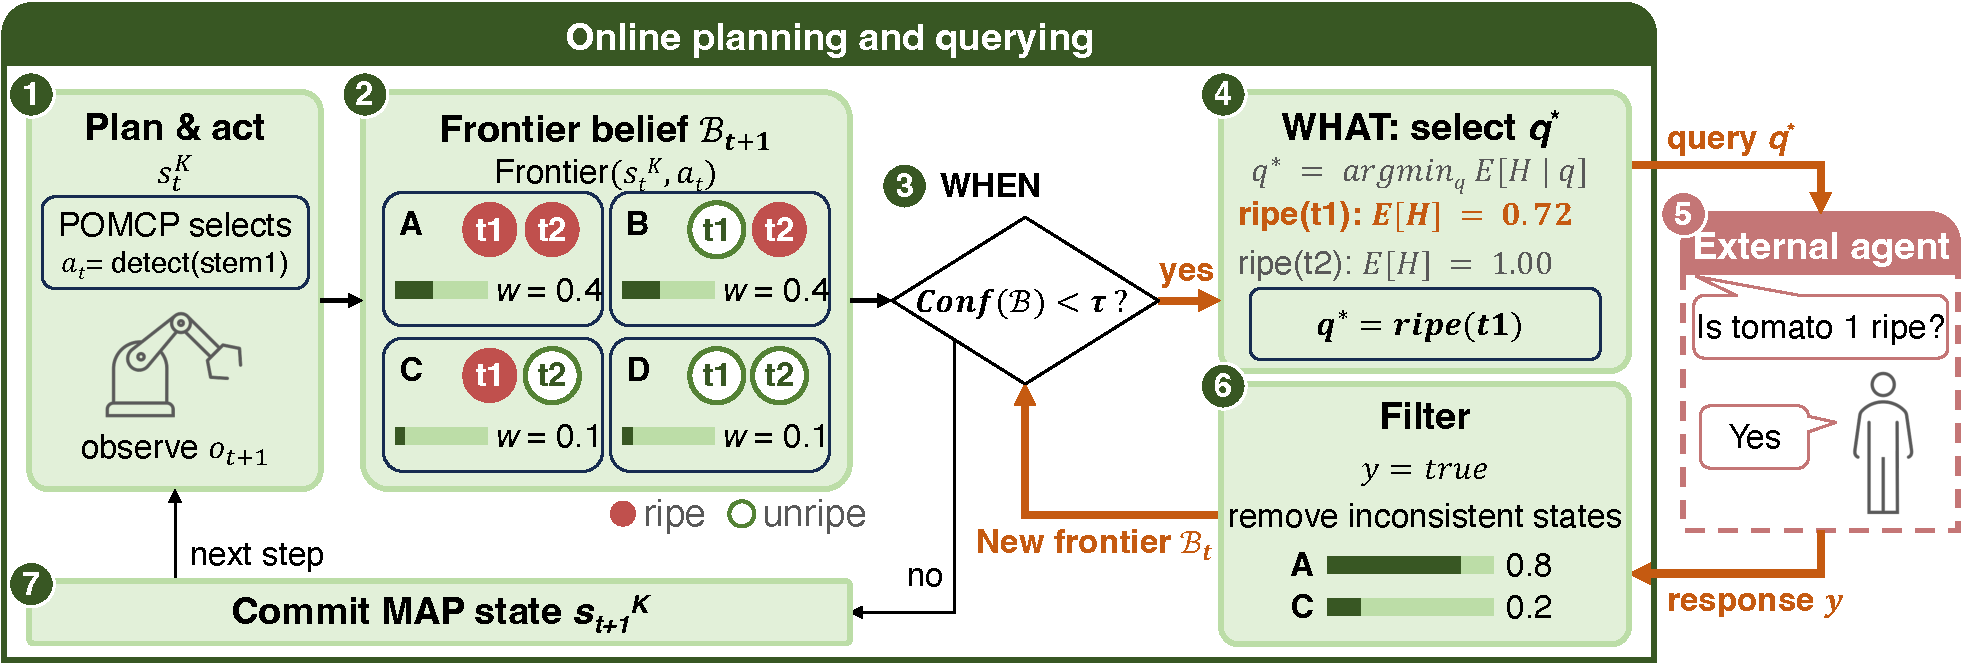
\includegraphics[width=0.995\linewidth]{figures/fig_method.pdf}
% \caption{Online planning and querying. If belief confidence falls below $\tau$, the robot queries the selected fact $q^*$ and uses the Boolean response $y\in\{\texttt{true},\texttt{false}\}$ to update the belief and knowledge base.}
% \label{fig:planning_and_query}
% \end{figure*}


\subsubsection{When to Query}~\label{method:when}\label{method:belief_rep}
To determine when to query, we \cp{compute confidence from normalized belief entropy~\citep{qu2023stochastic}, which decreases as probability concentrates on a single state.} We observe that a symbolic action usually changes only part of the state. For example, an action to pick a tomato can change which object the robot holds but preserves the robot location. We therefore define the \textit{frontier} of reachable successor states as $\mathrm{Frontier}(s_t^{K},a_t)=\{s_{t+1}^{1},\ldots,s_{t+1}^{j}\}$, \cp{where $s_{t+1}^{k}\neq s_{t+1}^{\ell}$ for all $k\neq\ell$.} We restrict particle sampling to the frontier instead of the entire symbolic state space.

As shown in Fig.~\ref{fig:planning_and_query}, we construct the weighted belief over the $j$ frontier states with normalized weights $w_k$.
Here, $\mathcal{B}_{t+1}=\{(s_{t+1}^{k},w_k)\}_{k=1}^{j}$, with $\sum_{k=1}^{j}w_k=1.$
Specifically, we compute these weights by normalizing the product of the transition probability from $s_t^{K}$ and the observation likelihood.
\begin{equation}
\begin{aligned}
\bar{w}_{k}&=T(s_{t+1}^{k}\mid s_t^{K},a_t)\,O(o_{t+1}\mid s_{t+1}^{k},a_t),\\
w_k&=\bar{w}_k/\sum_{\ell=1}^{j}\bar{w}_{\ell}.
\end{aligned}
\label{eq:belief_update}
\end{equation}
If all $\bar{w}_k$ are zero, we set $w_k=1/j$. We use the weighted frontier belief for confidence calculation and query selection. POMCP maintains sampled states in the search tree to estimate action values. Both components use the same symbolic transition and observation models.

We compute the entropy of the belief as
$\mathcal{H}(\mathcal{B}_{t+1}) = -\sum_{k=1}^{j}w_k\log_2 w_k.$
Because the maximum entropy depends on the number of represented worlds, we normalize by $\log_2 j$ and define
\begin{equation}
\mathrm{Conf}(\mathcal{B}_{t+1}) = 1-\frac{\mathcal{H}(\mathcal{B}_{t+1})}{\log_2 j}.
\label{eq:compute_confidence}
\end{equation}
For $j=1$, we define $\mathrm{Conf}(\mathcal{B}_{t+1})=1$. The score approaches zero if the represented states have similar weights and approaches one if most of the belief weight lies on one state.

Given a predefined threshold $\tau\in[0,1]$, the robot triggers a query if
$\mathrm{Conf}(\mathcal{B}_{t+1})<\tau.$
A higher threshold $\tau$ requires a more concentrated belief and can increase the number of queries.









\subsubsection{What to Query}~\label{method:what}
If belief confidence falls below $\tau$, the robot triggers a query and \cp{decides which fact to ask about}. \cp{Since an answer eliminates inconsistent frontier states}, we select the fact with the largest expected reduction in belief entropy.

\begin{algorithm}[t]
\caption{Planning and Querying}
\label{alg:online_planning}
\DontPrintSemicolon
\textbf{Input}\quad initial state $s_0^{K}$, goal condition $\mathcal{G}$, confidence threshold $\tau$, step limit $T_{\max}$\;
\textbf{Output}\quad executed action sequence $\pi$\;
\BlankLine
$\mathcal{B}\gets\{(s_0^{K},1)\}\qquad t\gets0\qquad \pi\gets()$\label{alg1_planning:initialize}\;
\While{$t<T_{\max}\land\mathcal{G}\nsubseteq s_t^{K}$}{
    \label{alg1_planning:termination}
    $a_t\gets$\Search{$\mathcal{B}$}\label{alg1_planning:search}\;
    \If{$a_t=\emptyset$}{
        \textbf{break}\label{alg1_planning:dead_end}\;
    }
    execute $a_t$ and receive $o_{t+1}$\label{alg1_planning:execute}\;
    $\pi\gets\pi\mathbin{\|}a_t$\label{alg1_planning:record}\;
    $\mathcal{B}\gets$\UpdateBelief{$s_t^{K},a_t,o_{t+1}$}\label{alg1_planning:belief_update}\hfill Eq.~\eqref{eq:belief_update}\;
    $c\gets\mathrm{Conf}(\mathcal{B})$\label{alg1_planning:compute_conf}\hfill Eq.~\eqref{eq:compute_confidence}\;
    \While{$c<\tau$}{
        $q^*\gets$\SelectBestHypothesis{$\mathcal{B}$}\label{alg1_planning:select_hypo}\hfill Eq.~\eqref{eq:select_hypo}\;
        \If{$q^*=\emptyset$}{
            \textbf{break}\label{alg1_planning:no_candidate}\;
        }
        $y\gets$\QuerySource{$q^*$}\label{alg1_planning:query}\;
        $\mathcal{B}\gets$\FilterBelief{$\mathcal{B},q^*,y$}\label{alg1_planning:filter}\hfill Eq.~\eqref{eq:filter}\;
        $c\gets\mathrm{Conf}(\mathcal{B})$\label{alg1_planning:recompute_conf}\hfill Eq.~\eqref{eq:compute_confidence}\;
    }
    $s_{t+1}^{K}\gets\arg\max_{s^k\in\mathcal{B}}w_k$\label{alg1_planning:commit}\;
    \cp{$\mathcal{B}\gets\{(s_{t+1}^{K},1)\}$}\label{alg1_planning:reset_belief}\;
    $t\gets t+1$\label{alg1_planning:advance}\;
}
\KwRet $\pi$\label{alg1_planning:return}\;
\end{algorithm}



Specifically, we define the query candidate set $\mathcal{Q}(\mathcal{B})$ by extracting atomic facts whose truth values differ across the remaining frontier states in the belief,
$\mathcal{Q}(\mathcal{B}) = \bigcup_{(s,w)\in\mathcal{B}}s \setminus \bigcap_{(s,w)\in\mathcal{B}}s.$
For each candidate fact $q\in\mathcal{Q}(\mathcal{B})$, we partition the belief according to whether $q$ holds in each state,
$\mathcal{B}^{q+}=\{(s^k,w_k)\mid q\in s^k\}$, $\mathcal{B}^{q-}=\{(s^k,w_k)\mid q\notin s^k\}.$
Let $P(q)=\sum_{k:q\in s^k}w_k$ and $P(\neg q)=1-P(q)$. Entropy within each subset is computed after conditionally normalizing its weights. The expected posterior entropy of asking about $q$ is
$\mathbb{E}[\mathcal{H}\mid q] = P(q)\mathcal{H}(\mathcal{B}^{q+}) + P(\neg q)\mathcal{H}(\mathcal{B}^{q-}).$
The selected query is
\begin{equation}~\label{eq:select_hypo}
q^* = \arg\min_{q\in\mathcal{Q}(\mathcal{B})} \left[P(q)\mathcal{H}(\mathcal{B}^{q+})+P(\neg q)\mathcal{H}(\mathcal{B}^{q-})\right].
\end{equation}
Eq.~\eqref{eq:select_hypo} selects the fact $q^*$ that maximizes expected entropy reduction. The robot then converts this fact into a binary query about the current state. For example, $q^*=\texttt{ripe}(\text{tomato}_1)$ produces the question \textit{`Is tomato 1 ripe?'}. Based on the response $y\in\{\texttt{true},\texttt{false}\}$, the robot updates the belief by removing states inconsistent with the reported truth value,
\begin{equation}
\mathcal{B}
\leftarrow
\begin{cases}
\{(s^k,w_k)\mid q^*\in s^k\}, & y=\texttt{true},\\
\{(s^k,w_k)\mid q^*\notin s^k\}, & y=\texttt{false}.
\end{cases}
\label{eq:filter}
\end{equation}
After each response, we renormalize the remaining weights, recompute confidence, and continue querying until confidence reaches \(\tau\) or no differentiating fact remains. We then use the MAP state \(s_{t+1}^{K} = \arg\max_{s^k\in\mathcal{B}_{t+1}}w_k\) \cp{for} symbolic planning and checking action preconditions. \cp{We also construct the next frontier from \(s_{t+1}^{K}\) and the next action rather than propagate the full posterior. By combining the query loop with the MAP approximation, we can limit the computational cost of belief updates while reducing the risk of committing to an incorrect state.}



% The robot renormalizes the retained weights, recomputes confidence, and selects another fact if confidence remains below $\tau$. The verification loop ends if confidence reaches $\tau$ or no differentiating fact remains. The robot then commits the maximum a posteriori state (MAP)
% $s_{t+1}^{K} = \arg\max_{s^k\in\mathcal{B}_{t+1}}w_k$
% for subsequent symbolic planning. To limit the computational cost of belief updates, we construct the next frontier from the committed knowledge state and the next action.

Alg.~\ref{alg:online_planning} explains the overall online planning and querying procedure. The robot first initializes the belief, step counter, and action sequence (line~\ref{alg1_planning:initialize}). Execution continues while $t<T_{\max}$ and the goal condition is not satisfied, $\mathcal{G}\nsubseteq s_t^{K}$ (line~\ref{alg1_planning:termination}). At each step, POMCP selects an action (line~\ref{alg1_planning:search}), and execution stops if no action is available (line~\ref{alg1_planning:dead_end}). Otherwise, the robot executes the action  (lines~\ref{alg1_planning:execute} and~\ref{alg1_planning:record}), then constructs the weighted frontier belief and computes confidence (lines~\ref{alg1_planning:belief_update} and~\ref{alg1_planning:compute_conf}). If confidence falls below $\tau$, the robot selects a candidate fact (line~\ref{alg1_planning:select_hypo}). If no candidate remains, the query loop ends (line~\ref{alg1_planning:no_candidate}). Otherwise, the robot queries an external agent, obtains an answer, and filters the belief (lines~\ref{alg1_planning:query} and~\ref{alg1_planning:filter}), then recomputes confidence (line~\ref{alg1_planning:recompute_conf}). After the query loop, the most probable remaining state becomes the next symbolic planning state (line~\ref{alg1_planning:commit}).

\begin{figure*}[t]
\captionsetup{skip=0pt}
\centering
% 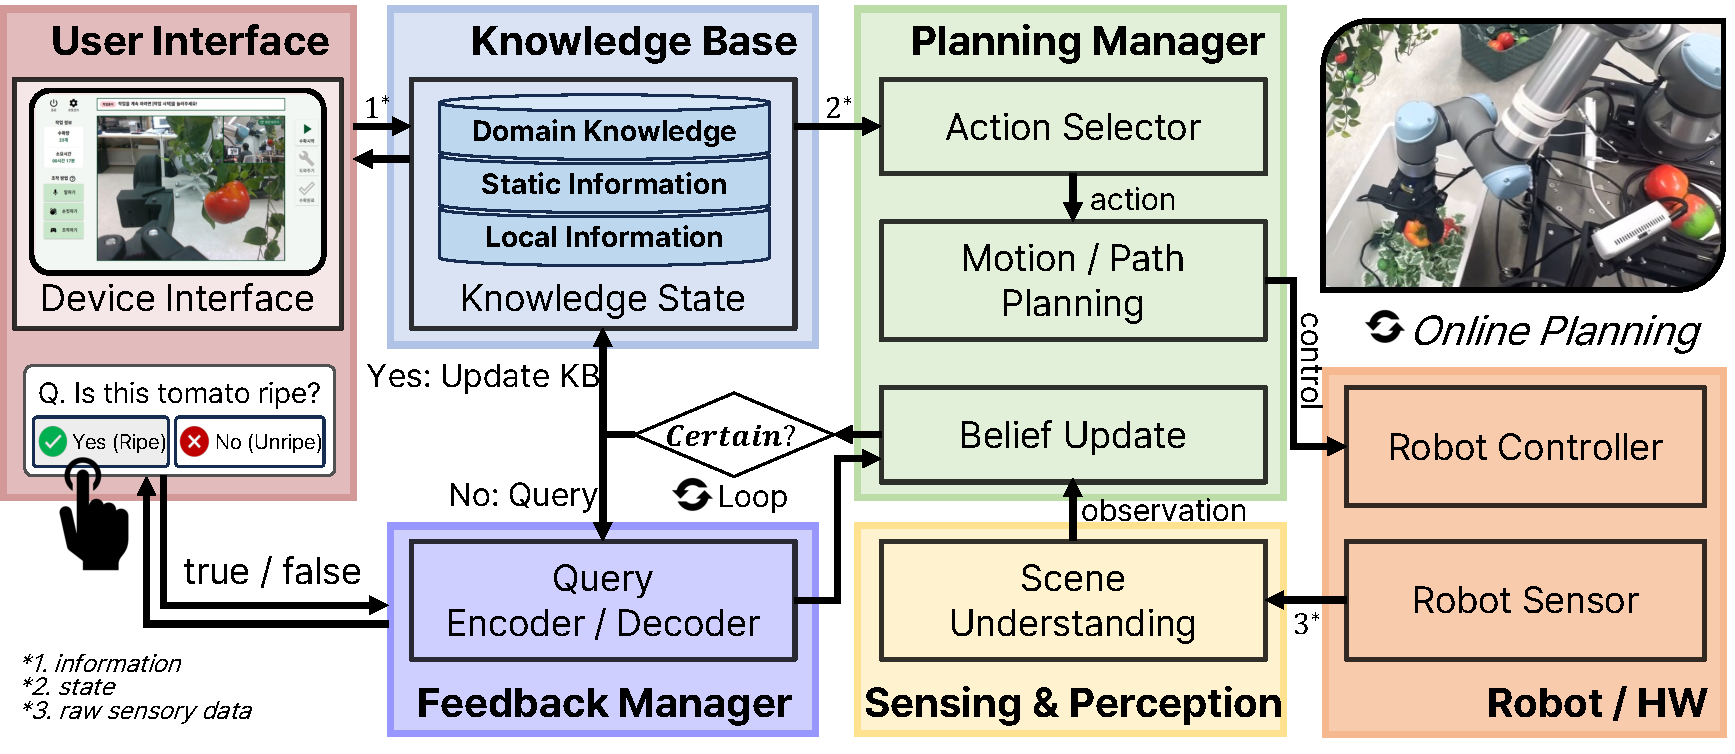
\includegraphics[width=0.95\linewidth]{figures/fig3_implementation.pdf}
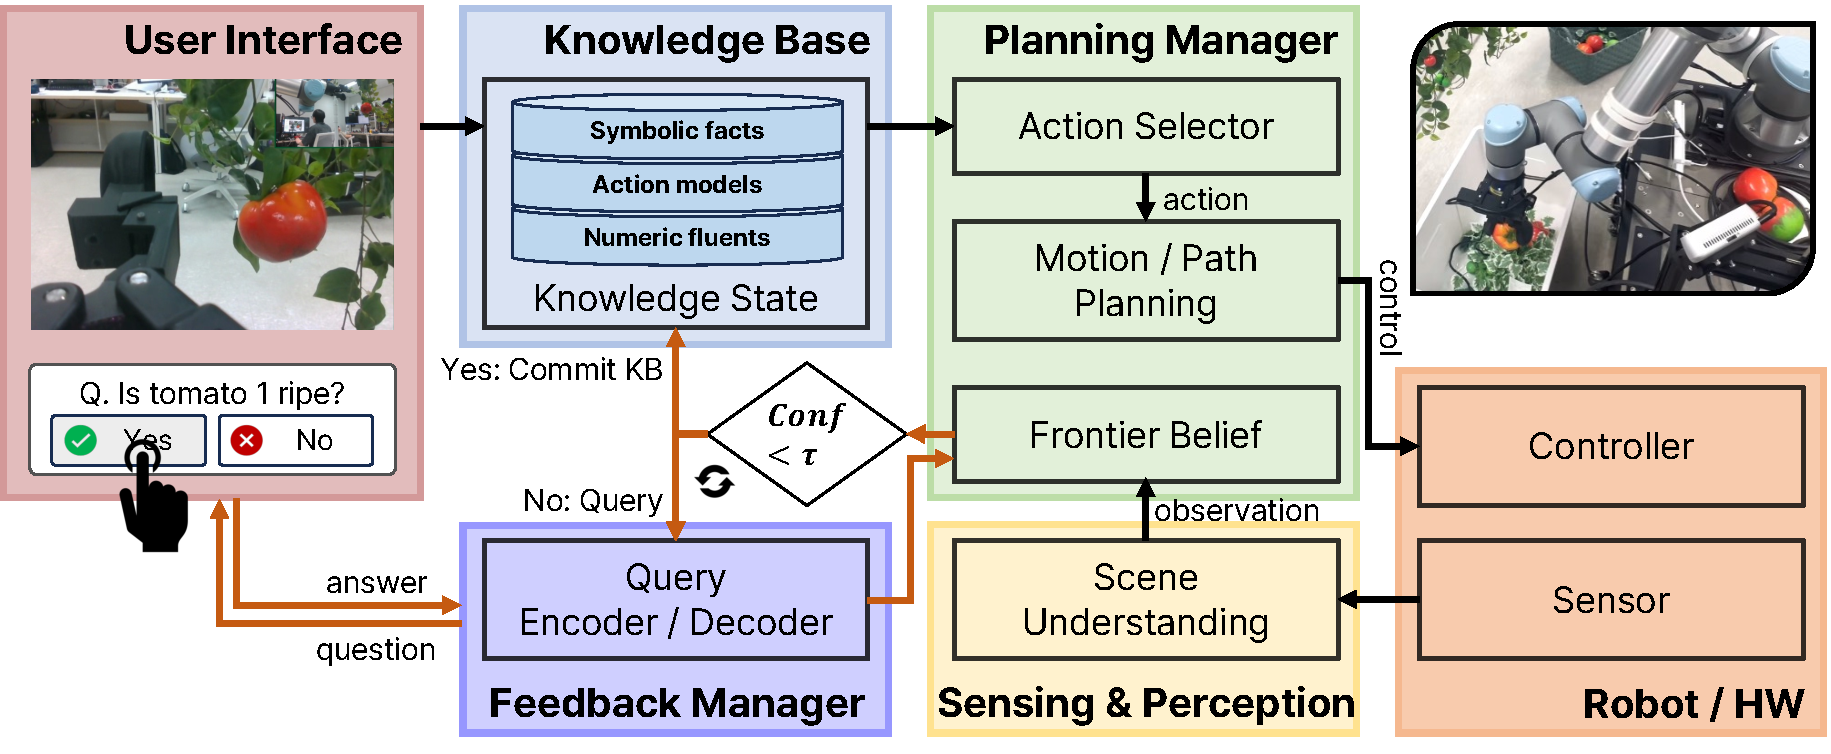
\includegraphics[width=0.95\linewidth]{figures/fig_architecture.pdf}
\caption{Framework for robot execution of the proposed planning and querying method. The Knowledge Base (KB) stores shared symbolic facts and action models, while Sensing and Perception (SP) supplies observations from robot sensors. The Planning Manager (PM) selects actions and determines queries. If belief confidence falls below $\tau$, the Feedback Manager (FM) converts the selected fact into a question that the User Interface (UI) presents to the human. The FM converts the response into Boolean evidence, which the PM uses to update the belief and continue planning.}\label{fig:data_flow}
\end{figure*}

\subsection{System Implementation}~\label{method:modules}
We implement a modular framework to execute the proposed planning and querying method on a robot, as shown in Fig.~\ref{fig:data_flow}. The Knowledge Base (KB) stores symbolic facts and action models, and Sensing and Perception (SP) provides observations and numeric state estimates from sensor data. The Planning Manager (PM) uses this information to select robot actions, construct the frontier belief, and decide when and what to query. The Feedback Manager (FM) converts the selected fact into a question and the response into evidence for the belief update. The User Interface (UI) presents the questions and collects responses during human interaction.

% \label{method:KB}
% The KB partitions information into domain knowledge $\mathcal{I}^{D}$, static structured information $\mathcal{I}^{S}$, and local information $\mathcal{I}^{L}$ obtained during execution.
% \[\mathcal{KB}=\mathcal{I}^{D}\sqcup\mathcal{I}^{S}\sqcup\mathcal{I}^{L}.\]
% Domain knowledge contains action schemas and task rules. Static information includes invariant facts and fixed map or robot parameters. Local information contains perceptual facts and numeric fluents that are updated during execution. SP maps raw sensor input to these task-level observations. For example, RGB-D sensing can update object pose and ripeness estimates, while the symbolic observation likelihood determines how those observations weight the frontier states.

\label{method:action_execution}
Each symbolic action invokes a robot skill. Actions such as $\texttt{navigate}(\text{robot},l_1,l_2)$ and $\texttt{pick}(\text{robot},\text{tomato}_1)$ specify task-level intentions, while an off-the-shelf motion planner such as MoveIt~\citep{chitta2012moveit} uses numeric fluents from the KB to generate low-level motion.

\label{method:FM}
The FM maps the selected predicate to a predefined question template and converts the response to a Boolean value. For example, the predicate $\mathrm{ripe}(t_1)$ is converted into the question ``Is tomato $t_1$ ripe?'' When interacting with human participants, the tablet UI displays the camera view, highlights the referenced object with a bounding box, and presents simple response options. Participants answer the question based on the displayed information, and the planner updates its belief and selects the next robot action accordingly.

\section{Experiments}~\label{experiment}
We evaluate our method in waste sorting (\textit{Sort}) and tomato harvesting (\textit{Harvest}) through a baseline comparison, an ablation study, and a confidence-threshold sweep. The baseline comparison evaluates complete planning systems that query an external agent. Oracle simulations compare Ours with KnowNo, IntroPlan, and POMCP-Q. Physical robot experiments compare Ours with KnowNo using VLM and human feedback to examine whether the performance trends persist across feedback sources. The ablation study examines the contributions of query timing and query selection in simulation. The threshold sweep examines the trade-off between task success and query count.

The oracle experiments include $200$ trials per domain and condition. The VLM experiments include $40$ trials per domain and method. The human evaluation involves five participants, with $10$ trials per domain and method and $40$ trials in total.

\begin{figure}[t]
    \centering
    \begin{subfigure}[t]{0.48\linewidth}
        \centering
        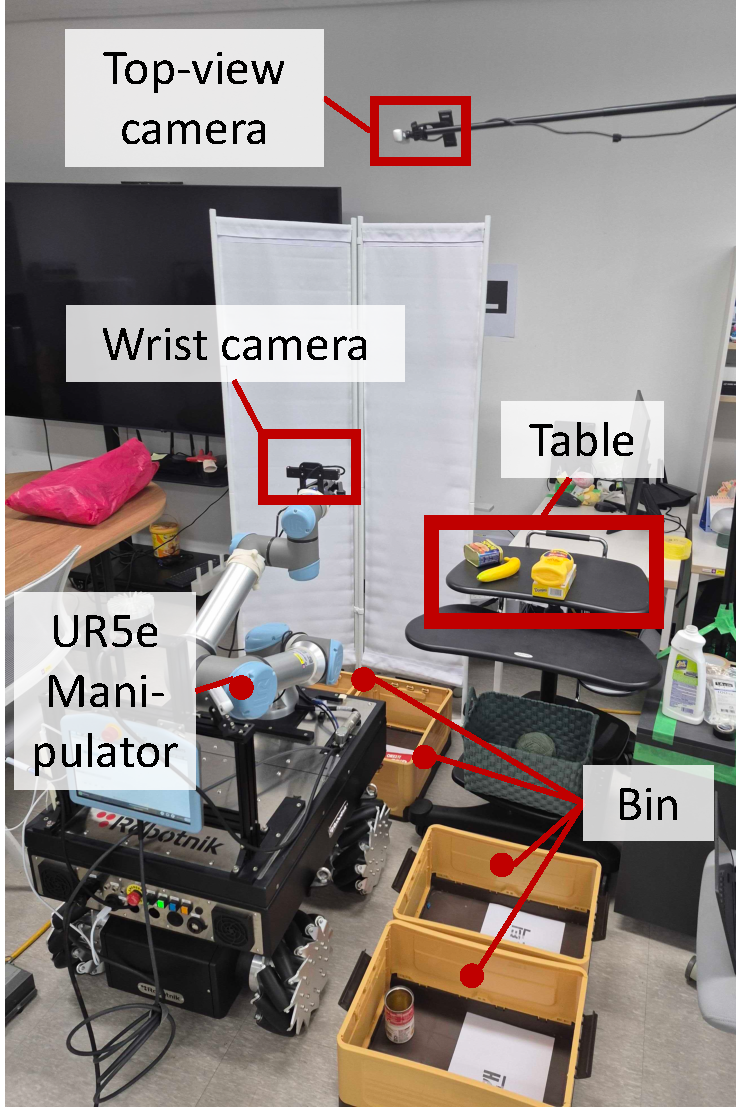
\includegraphics[width=\linewidth]{figures/03_SETUP/01_WasteSortingEnv.pdf}
        \caption{Sort}
        \label{fig:dom1}
    \end{subfigure}\hfill
    \begin{subfigure}[t]{0.48\linewidth}
        \centering
        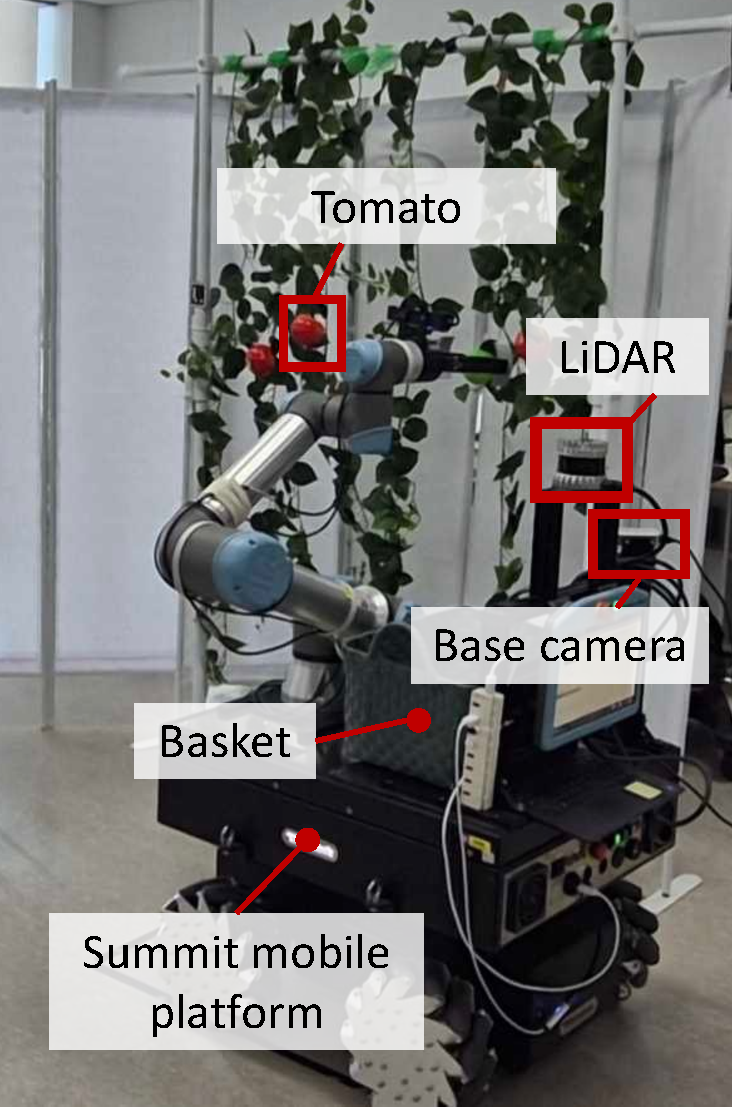
\includegraphics[width=\linewidth]{figures/03_SETUP/02_TomatoHarvestEnv.pdf}
        \caption{Harvest}
        \label{fig:dom2}
    \end{subfigure}
\caption{Physical robot setups for the two task domains. (a) Sort uses a fixed UR5e arm to sort objects into the appropriate bins. (b) Harvest uses a Summit mobile platform with a UR5e arm to navigate between tomato stems and harvest tomatoes. Annotations identify robot components, sensors, and task equipment.}    \label{fig:env_setting}
\end{figure}


\subsection{Experimental Setup}~\label{exp:setup}
The oracle experiments use simulated task execution and exact answers. The VLM and human experiments use physical robots in laboratory environments. Fig.~\ref{fig:env_setting} shows the physical setups. Sort uses a fixed UR5e robot arm. Harvest uses a Summit mobile platform equipped with a UR5e robot arm. The mobile platform uses an RGB-D camera for perception and LiDAR for localization. Sort uses SAM3 for object detection~\citep{carion2025sam3segmentconcepts}. Harvest uses YOLOv12 for object detection~\citep{tian2025yolov12}.


% \subsubsection{Task Domains}~\label{exp:setup_domains}
% The Sort task requires the robot to place every object in the correct bin. The UR5e robot is positioned between the objects and recycling bins in Fig.~\ref{fig:dom1}. All objects are within reach. The robot can detect objects and then pick and place them. Each object belongs to one of four waste categories corresponding to general waste or recyclable paper or cans or plastic. The categories are initially unknown. The main sources of uncertainty in this domain are occlusion and noisy sensor observations. In simulation we randomize the initial object arrangement for each trial. A trial succeeds if the robot places all objects in the correct bins within the step limit. Each correct placement yields a task reward of $+5$. Completion of the task yields an additional reward of $+10$. A penalty of $-10$ applies to the third and each subsequent detection action in a consecutive sequence.

% The Harvest task requires the robot to harvest fresh ripe tomatoes and discard rotten tomatoes. Four tomatoes are distributed across two stems in Fig.~\ref{fig:dom2}. The robot navigates between the docking station and the two stems. The \texttt{detect} action distinguishes ripe from unripe tomatoes. After a tomato is picked the \texttt{scan} action distinguishes fresh from rotten tomatoes. The robot uses \texttt{place} for fresh tomatoes and \texttt{discard} for rotten tomatoes. Unripe tomatoes remain on the stem. The main source of uncertainty in this domain is noisy sensor observations. In simulation we randomize tomato locations across the two stems for each trial. A trial succeeds if all fresh ripe tomatoes are harvested and all rotten tomatoes are discarded within the step limit. Correct placement of a fresh tomato or disposal of a rotten tomato yields a task reward of $+10$. Consecutive \texttt{detect} actions at the same stem and consecutive \texttt{scan} actions on the same tomato incur a penalty of $-5$ from the second action onward.


\subsubsection{Task Domains}~\label{exp:setup_domains}
We evaluate two domains with different sources of uncertainty (Fig.~\ref{fig:env_setting}). In Sort, the robot detects, picks, and places objects into bins for four waste categories. Object categories are initially unknown, and occlusion and noisy observations create uncertainty about object presence and category. In Harvest, the robot navigates between two stems to harvest fresh ripe tomatoes and discard rotten ones, leaving unripe tomatoes untouched. Detection estimates ripeness, while scanning after picking distinguishes fresh from rotten tomatoes. Noisy observations create uncertainty about tomato state.



\subsubsection{Implementation Details}~\label{exp:details}
Our POMCP planner uses $100$ simulations per planning step with a maximum simulation depth of $20$. The discount factor is $\gamma=0.2$ and the UCB exploration constant is $c=1.0$. The default confidence threshold is $\tau=0.8$. We use Gemma 4 31B IT with NVFP4 quantization~\citep{gemmateam2026gemma4} as the external agent in the VLM experiments. Appendix~\ref{appx:settings} provides the baseline configurations and additional experimental details.

\subsubsection{Evaluation Metrics}~\label{exp:metrics}
We compute success rate as the fraction of all trials in which the robot achieves the task goal. In the oracle experiments, we allow at most $20$ physical actions per trial. For POMCP-Q, we also allow at most $30$ queries per trial. Query count is the number of queries per trial. Query probability is the fraction of physical steps that trigger at least one query. Plan length is the number of physical actions executed per trial. Planning time is the cumulative time spent on plan search per trial. Interaction time is the cumulative time spent on query and response per trial. We measure total time as the elapsed time per physical trial, including planning, robot execution, and interaction. For oracle trials, we report planning time as total time. We report interaction time only for the VLM and human experiments. For all metrics other than success rate, we report the mean and sample standard deviation across successful trials.

% Numerical reference: asset/BRL_EXP/05; originals retained in 05_exp_system.tex.
\subsection{System Evaluation}~\label{exp:sys_eval}
\begin{table}[t]
\centering
\captionsetup{font=small,skip=5pt}
\caption{Query \textbf{timing} (when) and query \textbf{selection} (what) strategies. KnowNo, IntroPlan and POMCP-Q are the baselines. R, S1--S2 and T1--T3 are the ablation configurations. A dash denotes a combination not evaluated in this study.}
\label{tab:query_strategy_matrix}
\footnotesize
\setlength{\tabcolsep}{1pt}
\renewcommand{\arraystretch}{1.15}
\arrayrulecolor{black}
\begin{tabular*}{\columnwidth}{@{\extracolsep{\fill}}lcccc@{}}
\toprule
\diagbox[innerwidth=\widthof{Conformal Set},height=0.85cm,dir=NW,linewidth=0.3pt,font=\bfseries]{What}{When} & Random & \makecell[c]{Conformal\\Prediction} & \makecell[c]{Reward-\\based} & Confidence \\
\midrule
Random & R & -- & -- & S1 \\
\addlinespace[3pt]
Conformal Set & -- & \makecell[c]{KnowNo,\\IntroPlan} & -- & -- \\
\addlinespace[3pt]
Reward-based & -- & -- & POMCP-Q & S2 \\
\addlinespace[3pt]
Entropy Gain & T1 & T2 & T3 & \textbf{Ours} \\
\bottomrule
\end{tabular*}
\end{table}

Table~\ref{tab:query_strategy_matrix} summarizes the baseline and ablation configurations. The baseline comparison in Sec.~\ref{exp:sys_baseline} evaluates KnowNo, IntroPlan, and POMCP-Q against Ours. This comparison evaluates complete task planning systems that query an external agent to plan and execute actions. We evaluate these systems with oracle, VLM, and human feedback to examine whether the observed performance trends persist across feedback sources. The ablation study in Sec.~\ref{exp:policy_ablation} evaluates R, S1--S2, and T1--T3 against Ours where T1--T3 examine query timing (when) and S1--S2 examine query selection (what). Finally the threshold study in Sec.~\ref{exp:sys_threshold} examines how the confidence threshold affects task success and query count. Both the ablation and threshold studies use oracle responses in simulation.



\subsubsection{Baseline Comparison}~\label{exp:sys_baseline}
\noindent\textbf{Oracle}. The oracle comparison includes three baselines with the query timing and selection strategies summarized in Table~\ref{tab:query_strategy_matrix}. KnowNo~\citep{ren2023robots} requests an action choice if its conformal prediction set does not specify a single ordinary action. IntroPlan~\citep{liang2024introspective} extends KnowNo and incorporates retrieved examples and explanations into candidate evaluation before it requests an action choice. We implement a HARPS-inspired POMCP baseline (POMCP-Q)~\citep{burks2023harps} that selects between physical actions and Boolean queries to an external agent by maximizing expected cumulative reward. We adapt HARPS to our symbolic task domains, executing physical actions and queries separately. Table~\ref{tab:baseline_results} and Fig.~\ref{fig:baseline_results} compare the four methods.

\begin{figure*}[!tp]
\centering
\begin{subfigure}[t]{0.247\textwidth}
\centering
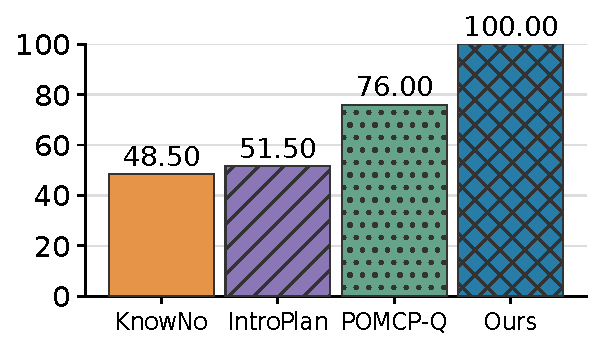
\includegraphics[width=\linewidth,height=.16\textheight,keepaspectratio]{figures/04_ORACLE_BASELINE/exp_oracle_waste_success.pdf}
\caption{Sort Success rate (\%)}
\label{fig:baseline_oracle_waste_success}
\end{subfigure}%
\hspace{0.004\textwidth}%
\begin{subfigure}[t]{0.247\textwidth}
\centering
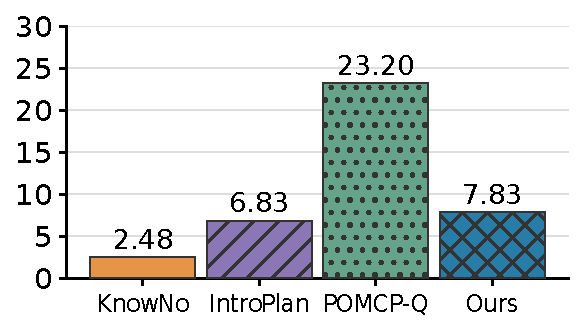
\includegraphics[width=\linewidth,height=.16\textheight,keepaspectratio]{figures/04_ORACLE_BASELINE/exp_oracle_waste_queries.pdf}
\caption{Sort Query count}
\label{fig:baseline_oracle_waste_queries}
\end{subfigure}%
\hspace{0.004\textwidth}%
\begin{subfigure}[t]{0.247\textwidth}
\centering
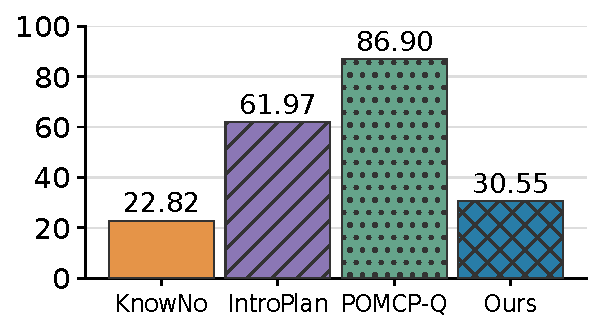
\includegraphics[width=\linewidth,height=.16\textheight,keepaspectratio]{figures/04_ORACLE_BASELINE/exp_oracle_waste_query_probability.pdf}
\caption{Sort Query prob. (\%)}
\label{fig:baseline_oracle_waste_query_probability}
\end{subfigure}%
\hspace{0.004\textwidth}%
\begin{subfigure}[t]{0.247\textwidth}
\centering
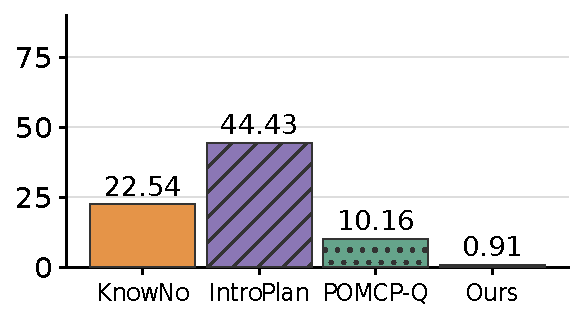
\includegraphics[width=\linewidth,height=.16\textheight,keepaspectratio]{figures/04_ORACLE_BASELINE/exp_oracle_waste_plan_time.pdf}
\caption{Sort Plan time (s)}
\label{fig:baseline_oracle_waste_plan_time}
\end{subfigure}
\par\smallskip
\begin{subfigure}[t]{0.247\textwidth}
\centering
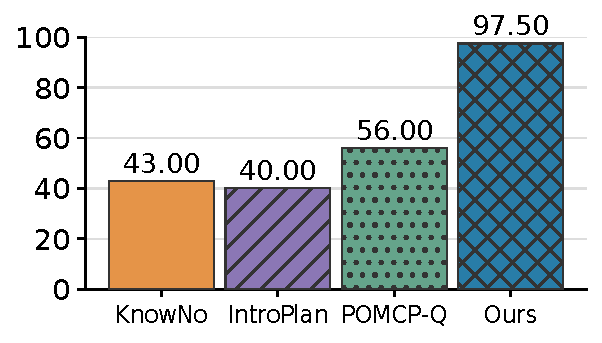
\includegraphics[width=\linewidth,height=.16\textheight,keepaspectratio]{figures/04_ORACLE_BASELINE/exp_oracle_tomato_success.pdf}
\caption{Harvest Success rate (\%)}
\label{fig:baseline_oracle_tomato_success}
\end{subfigure}%
\hspace{0.004\textwidth}%
\begin{subfigure}[t]{0.247\textwidth}
\centering
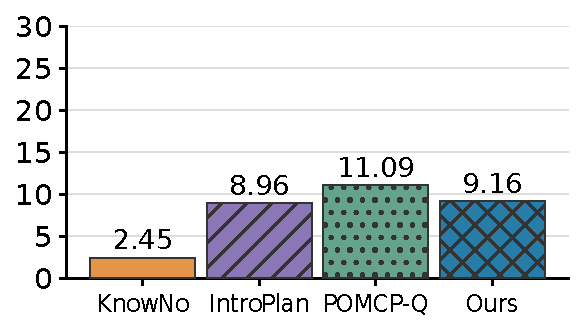
\includegraphics[width=\linewidth,height=.16\textheight,keepaspectratio]{figures/04_ORACLE_BASELINE/exp_oracle_tomato_queries.pdf}
\caption{Harvest Query count}
\label{fig:baseline_oracle_tomato_queries}
\end{subfigure}%
\hspace{0.004\textwidth}%
\begin{subfigure}[t]{0.247\textwidth}
\centering
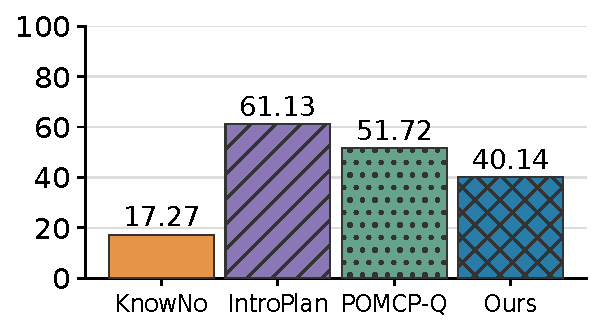
\includegraphics[width=\linewidth,height=.16\textheight,keepaspectratio]{figures/04_ORACLE_BASELINE/exp_oracle_tomato_query_probability.pdf}
\caption{Harvest Query prob. (\%)}
\label{fig:baseline_oracle_tomato_query_probability}
\end{subfigure}%
\hspace{0.004\textwidth}%
\begin{subfigure}[t]{0.247\textwidth}
\centering
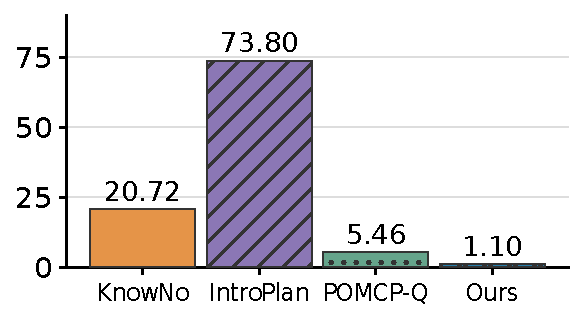
\includegraphics[width=\linewidth,height=.16\textheight,keepaspectratio]{figures/04_ORACLE_BASELINE/exp_oracle_tomato_plan_time.pdf}
\caption{Harvest Plan time (s)}
\label{fig:baseline_oracle_tomato_plan_time}
\end{subfigure}
\caption{Oracle baseline comparison. (a), (e) Ours achieves the highest success rates in both domains. (b)-(c), (f)-(g) Ours uses more queries than KnowNo and IntroPlan but fewer than POMCP-Q, with a lower query probability than IntroPlan and POMCP-Q. (d), (h) Ours has the shortest plan times in both domains. These results indicate that query count alone does not explain task success or plan time.}
\label{fig:baseline_results}
\end{figure*}





% As shown in Table~\ref{tab:baseline_results} and Fig.~\ref{fig:baseline_results}, our method achieves the highest success rate in both domains. It completes all $200$ Sort trials and $196$ of $200$ Harvest trials. Our method achieves success rates of $100.00\%$ in Sort and $98.00\%$ in Harvest compared with $87.00\%$ and $57.50\%$ for POMCP-Q. The mean query counts are also lower at $7.83$ and $9.16$ compared with $24.52$ and $11.28$ for POMCP-Q. Two factors may explain the lower success rate and higher query count of POMCP-Q. First, query actions expand the action space so POMCP must evaluate more alternatives within the same simulation budget. Second, expected task reward does not explicitly measure confidence in the current state. Our method selects queries at the observation stage and restricts POMCP planning to physical actions. These results show that a higher query count alone does not guarantee a higher success rate.

% Compared to KnowNo and IntroPlan, our method uses more queries. Their mean query counts are $2.48$ and $6.83$ in Sort compared with $7.83$ for our method. In Harvest, the corresponding counts are $2.45$ and $8.96$ compared with $9.16$ for our method. This difference in query count arises from how each method handles a query trigger. If a query is triggered, our method repeats queries until belief confidence reaches $\tau$. KnowNo and IntroPlan ask only one question per trigger. Therefore our method can use more queries despite a lower query probability than IntroPlan. However KnowNo and IntroPlan achieve success rates of only $48.50\%$ and $51.50\%$ in Sort and $43.00\%$ and $40.00\%$ in Harvest. Therefore a system is not necessarily better simply because it uses fewer queries.

% Plan time is also lowest for Ours in both domains despite the additional queries compared with KnowNo and IntroPlan. In Sort, mean plan time is $0.91$ seconds for Ours compared with $22.54$ seconds for KnowNo, $44.43$ seconds for IntroPlan, and $10.47$ seconds for POMCP-Q. In Harvest, the corresponding values are $1.10$, $20.72$, $73.80$, and $5.55$ seconds. KnowNo and IntroPlan require language-model inference for candidate generation and scoring at each planning step. IntroPlan performs additional reasoning and candidate evaluation, which increases inference time compared with KnowNo. Ours evaluates query timing and selection from the belief state and searches only over physical actions. The smaller search space supports faster planning than POMCP-Q. The time comparisons suggest that belief-based search can reduce plan time without repeated language-model inference. % Therefore a higher query count does not necessarily imply a higher planning cost.

% Our method combines confidence-based query timing with entropy gain query selection and achieves the highest success rate in both domains. The baseline comparisons suggest that effective query timing and selection are more important than query count alone.

As shown in Table~\ref{tab:baseline_results} and Fig.~\ref{fig:baseline_results}, Ours achieves success rates of $100.00\%$ in Sort and $97.50\%$ in Harvest, compared with $76.00\%$ and $56.00\%$ for POMCP-Q, while using fewer queries in both domains. POMCP-Q includes queries in the action space, increasing the alternatives evaluated within a fixed simulation budget. Its reward criterion also does not explicitly assess confidence in the current state. These differences may contribute to its lower success rate and higher query count. Ours verifies state facts after observations and restricts action planning to physical actions.

Ours uses more queries than KnowNo and IntroPlan because it continues verification until belief confidence reaches $\tau$, whereas both baselines request one action choice per trigger. This distinction explains how Ours can have a lower query probability than IntroPlan while asking more questions overall. Similar query counts also yield substantially different outcomes. In Harvest, IntroPlan and Ours use $8.96$ and $9.16$ queries, respectively, yet achieve success rates of $40.00\%$ and $97.50\%$. Query count alone therefore does not explain task success.

Ours also has the lowest plan time in both domains. KnowNo and IntroPlan invoke a language model for candidate generation and scoring, with IntroPlan additionally generating explanations for candidate evaluation. Ours computes query timing and selection from the belief state and searches over physical actions only. This avoids repeated language-model inference and limits the search space compared with POMCP-Q.



\begin{table*}[t]
\centering
\caption{Baseline results. Underlines mark best means.}
\label{tab:baseline_results}
\footnotesize
\setlength{\tabcolsep}{2pt}
\renewcommand{\arraystretch}{1.05}
\setlength{\extrarowheight}{0pt}
\medmuskip=1mu\relax
\begin{tabular*}{\textwidth}{@{\extracolsep{\fill}}llccccccc@{}}
% \begin{tabular}{llcccc}
\toprule
Setting & Method & Success (\%) & Query count & Query prob.(\%) & Plan length & Total time (s) & Inter. time (s) & Plan time (s)\\
\midrule
\multirow{4}{*}{\shortstack[l]{Oracle\\Sort}} & KnowNo & 48.50 & $\underline{2.48} \pm 1.42$ & $\underline{22.82} \pm 12.61$ & $10.78 \pm 1.35$ & $22.54 \pm 3.04$ & - & $22.54 \pm 3.04$ \\
 & IntroPlan & 51.50 & $6.83 \pm 1.53$ & $61.97 \pm 9.35$ & $10.99 \pm 1.49$ & $44.43 \pm 8.05$ & - & $44.43 \pm 8.05$ \\
 & POMCP-Q & 76.00 & $23.20 \pm 4.39$ & $86.90 \pm 5.29$ & $11.72 \pm 1.49$ & $10.16 \pm 1.36$ & - & $10.16 \pm 1.36$ \\
 & \textbf{Ours} & \textbf{\underline{100.00}} & $\boldsymbol{7.83 \pm 2.16}$ & $\boldsymbol{30.55 \pm 10.41}$ & $\boldsymbol{\underline{10.35} \pm 0.88}$ & $\boldsymbol{\underline{0.91} \pm 0.09}$ & - & $\boldsymbol{\underline{0.91} \pm 0.09}$ \\
\addlinespace[3pt]
\multirow{4}{*}{\shortstack[l]{Oracle\\Harvest}} & KnowNo & 43.00 & $\underline{2.45} \pm 1.06$ & $\underline{17.27} \pm 6.67$ & $14.01 \pm 1.07$ & $20.72 \pm 2.25$ & - & $20.72 \pm 2.25$ \\
 & IntroPlan & 40.00 & $8.96 \pm 2.04$ & $61.13 \pm 10.77$ & $14.61 \pm 1.46$ & $73.80 \pm 8.96$ & - & $73.80 \pm 8.96$ \\
 & POMCP-Q & 56.00 & $11.09 \pm 3.59$ & $51.72 \pm 10.50$ & $14.77 \pm 1.36$ & $5.46 \pm 1.11$ & - & $5.46 \pm 1.11$ \\
 & \textbf{Ours} & \textbf{\underline{97.50}} & $\boldsymbol{9.16 \pm 1.91}$ & $\boldsymbol{40.14 \pm 4.50}$ & $\boldsymbol{\underline{13.93} \pm 1.03}$ & $\boldsymbol{\underline{1.10} \pm 0.16}$ & - & $\boldsymbol{\underline{1.10} \pm 0.16}$ \\
\specialrule{0.4pt}{\aboverulesep}{1pt}\specialrule{0.4pt}{0pt}{\belowrulesep}
\multirow{2}{*}{\shortstack[l]{VLM\\Sort}} & KnowNo & 50.00 & $\underline{3.15} \pm 0.88$ & $28.64 \pm 7.96$ & $\underline{11.00} \pm 0.00$ & $\underline{186.51} \pm 10.90$ & $\underline{15.46} \pm 4.45$ & $19.99 \pm 4.76$ \\
 & \textbf{Ours} & \textbf{\underline{92.50}} & $\boldsymbol{6.70 \pm 1.76}$ & $\boldsymbol{\underline{19.81} \pm 3.27}$ & $\boldsymbol{11.24 \pm 0.49}$ & $\boldsymbol{193.69 \pm 13.52}$ & $\boldsymbol{26.83 \pm 7.76}$ & $\boldsymbol{\underline{0.99} \pm 0.05}$ \\
\addlinespace[3pt]
\multirow{2}{*}{\shortstack[l]{VLM\\Harvest}} & KnowNo & 25.00 & $\underline{7.20} \pm 1.87$ & $44.10 \pm 7.51$ & $16.10 \pm 1.73$ & $217.82 \pm 17.78$ & $44.99 \pm 13.10$ & $26.90 \pm 3.07$ \\
 & \textbf{Ours} & \textbf{\underline{92.50}} & $\boldsymbol{8.51 \pm 1.52}$ & $\boldsymbol{\underline{37.63} \pm 3.04}$ & $\boldsymbol{\underline{13.27} \pm 0.77}$ & $\boldsymbol{\underline{180.39} \pm 11.18}$ & $\boldsymbol{\underline{34.12} \pm 7.62}$ & $\boldsymbol{\underline{1.38} \pm 0.19}$ \\
\specialrule{0.4pt}{\aboverulesep}{1pt}\specialrule{0.4pt}{0pt}{\belowrulesep}
\multirow{2}{*}{\shortstack[l]{Human\\Sort}} & KnowNo & 20.00 & $\underline{3.00} \pm 1.41$ & $25.76 \pm 10.71$ & $11.50 \pm 0.71$ & $\underline{184.48} \pm 24.08$ & $\underline{11.59} \pm 7.94$ & $16.94 \pm 0.39$ \\
 & \textbf{Ours} & \textbf{\underline{90.00}} & $\boldsymbol{7.11 \pm 1.83}$ & $\boldsymbol{\underline{18.18} \pm 0.00}$ & $\boldsymbol{\underline{11.00} \pm 0.00}$ & $\boldsymbol{190.15 \pm 50.72}$ & $\boldsymbol{36.49 \pm 47.55}$ & $\boldsymbol{\underline{0.94} \pm 0.04}$ \\
\addlinespace[3pt]
\multirow{2}{*}{\shortstack[l]{Human\\Harvest}} & KnowNo & 30.00 & $\underline{3.67} \pm 0.58$ & $\underline{28.21} \pm 4.44$ & $\underline{13.00} \pm 0.00$ & $195.50 \pm 8.26$ & $\underline{19.04} \pm 8.16$ & $23.52 \pm 1.21$ \\
 & \textbf{Ours} & \textbf{\underline{100.00}} & $\boldsymbol{8.50 \pm 1.78}$ & $\boldsymbol{37.36 \pm 3.74}$ & $\boldsymbol{13.10 \pm 0.32}$ & $\boldsymbol{\underline{180.02} \pm 13.14}$ & $\boldsymbol{23.89 \pm 13.47}$ & $\boldsymbol{\underline{1.32} \pm 0.08}$ \\
\bottomrule
\end{tabular*}
\end{table*}












\vspace{10pt}
\noindent\textbf{VLM}\label{exp:vlm_eval}.
We evaluate whether the oracle trends persist with VLM feedback on physical robots.\footnote{Appendix~\ref{appx:vlm_prompts} provides the VLM prompts.} We select KnowNo because it achieves success rates similar to IntroPlan with fewer queries than either IntroPlan or POMCP-Q in the oracle experiments. The physical experiments compare task success and interaction costs between Ours and KnowNo. We conduct $40$ trials per method and domain. Fig.~\ref{fig:physical_results} presents the results.

\begin{figure*}[!tp]
\centering
\captionsetup[subfigure]{font=footnotesize,skip=1pt}
\begin{subfigure}[b]{0.49\textwidth}
\centering
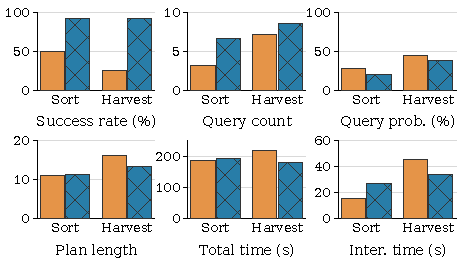
\includegraphics[width=\linewidth]{figures/05_PHYSICAL_BASELINE/exp_physical_vlm_group.pdf}
\caption{VLM responses}
\label{fig:physical_vlm}
\end{subfigure}%
\makebox[0.02\textwidth][c]{%
\raisebox{6pt}[0pt][0pt]{
\includegraphics[height=8pt]{figures/05_PHYSICAL_BASELINE/exp_physical_legend.pdf}}}%
\begin{subfigure}[b]{0.49\textwidth}
\centering
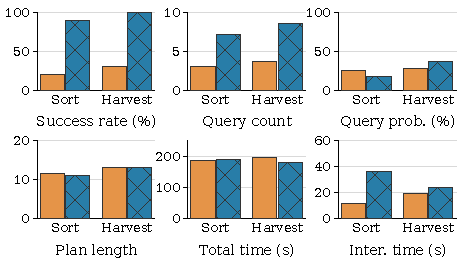
\includegraphics[width=\linewidth]{figures/05_PHYSICAL_BASELINE/exp_physical_human_group.pdf}
\caption{Human responses}
\label{fig:physical_human}
\end{subfigure}
\caption{Physical robot evaluation with VLM and human responses. (a) With VLM feedback, Ours achieves higher task success than KnowNo in both domains. (b) The same success advantage holds with human feedback.}
\label{fig:physical_results}
\end{figure*}



% \begin{table*}[t]
% \centering
% \caption{Physical robot results with VLM and human responses. Parentheses give successful trials over all trials. Other metrics report means over successful trials. A dash marks human results that are not yet available.}
% \label{tab:physical_robot_results}
% \small
% \setlength{\tabcolsep}{2.5pt}
% \begin{tabular*}{\textwidth}{@{\extracolsep{\fill}}lllccccccc}
% \toprule
% Source & Domain & Method & Success (\%) & \shortstack{Query\\count} & \shortstack{Query\\prob. (\%)} & \shortstack{Plan\\length} & \shortstack{Total\\time (s)} & \shortstack{Interaction\\time (s)} & \shortstack{Planning\\time (s)} \\
% \midrule
% VLM & Sort & KnowNo & 50.00 (20/40) & 3.15 & 28.64 & 11.00 & 186.51 & 15.46 & 20.08 \\
%  &  & Ours & 92.50 (37/40) & 6.70 & 19.81 & 11.24 & 193.69 & 26.83 & 1.11 \\
% \addlinespace
%  & Harvest & KnowNo & 25.00 (10/40) & 7.20 & 44.10 & 16.10 & 217.82 & 44.99 & 27.68 \\
%  &  & Ours & 92.50 (37/40) & 8.51 & 37.63 & 13.27 & 180.39 & 34.12 & 1.48 \\
% \midrule
% Human & Sort & KnowNo & 20.00 (2/10) & 2.90 & 26.09 & 11.50 & 184.48 & 11.59 & 16.94 \\
%  &  & Ours & 90.00 (9/10) & 7.20 & 18.18 & 11.00 & 190.15 & 36.49 & 0.94 \\
% \addlinespace
%  & Harvest & KnowNo & 30.00 (3/10) & 3.67 & 28.21 & 13.00 & 195.50 & 19.04 & 23.52 \\
%  &  & Ours & 10.00 (10/10) & 8.50 & 37.40 & 13.10 & 180.02 & 23.89 & 1.32 \\
% \bottomrule
% \end{tabular*}
% \end{table*}



Ours achieves $92.50\%$ success in both domains, compared with $50.00\%$ and $25.00\%$ for KnowNo in Sort and Harvest, respectively. Ours also requires less search time in both domains. Among successful Harvest trials, KnowNo uses $7.20$ queries compared with $8.51$ for Ours, yet executes longer plans and requires more total time, averaging $217.82$ seconds compared with $180.39$ seconds. In Sort, Ours achieves higher success but requires more time among successful trials. Mean total time is $193.69$ seconds for Ours and $186.51$ seconds for KnowNo. Mean interaction time is also longer at $26.83$ seconds compared with $15.46$ seconds. Ours therefore improves task success in both domains, while its advantage in total time is limited to Harvest. Query count alone does not explain total task time.
% Fewer queries therefore do not necessarily reduce execution costs.

We distinguish VLM response errors from planner failures. All three failures of Ours in each domain involve incorrect VLM feedback. In Sort, KnowNo has three VLM response failures and $17$ planner failures, with the latter involving autonomous action selections despite unmet preconditions. In Harvest, KnowNo has $18$ VLM response failures and $12$ planner failures. Six VLM failures involve repeated detection choices that exhaust the step limit despite feasible alternatives, and the remaining $12$ involve incorrect action selections.

These failures illustrate the importance of both query timing and query content. A single predicted action can still require state verification before execution. To select the correct action, the VLM must assess robot location, object states, and action preconditions. However, the VLM may still select an infeasible action or one that does not advance the task. Ours asks the VLM to verify current state facts and uses the updated belief for subsequent planning, leaving action selection to the planner.



% \begin{figure}[t]
% \centering
% 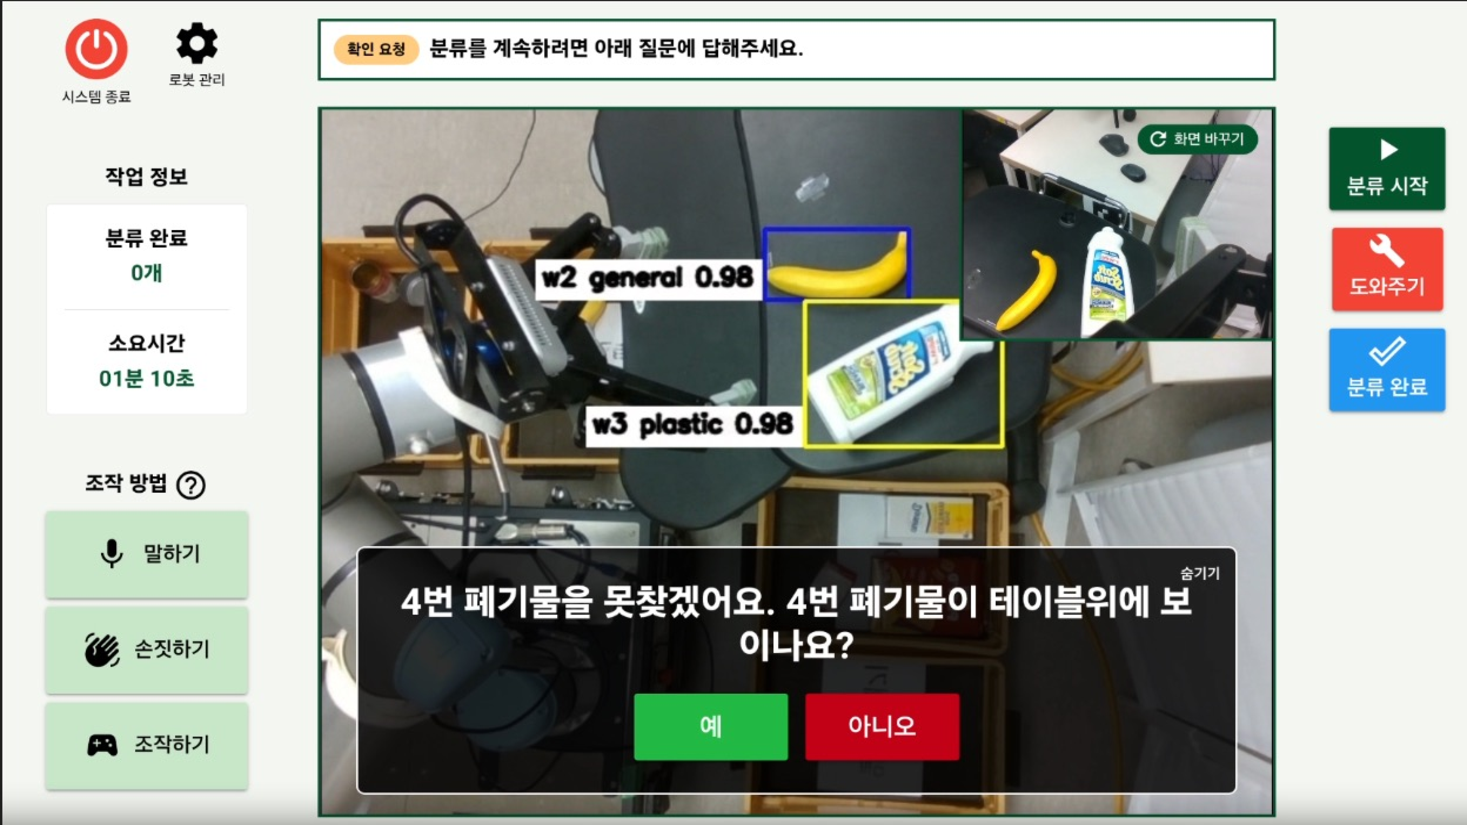
\includegraphics[width=\linewidth]{figures/exp_human_ui.pdf}
% \caption{Tablet interface used in the human evaluation. Participants view the robot camera feeds and select responses to robot queries.}
% \label{fig:human_tablet_interface}
% \end{figure}










\vspace{10pt}
\noindent\textbf{Human}\label{exp:human_eval}. 
We evaluate whether the oracle and VLM trends persist with human feedback using the same robot platforms and task domains. We recruited five participants (one man and four women), with a mean age of $26.4$ years (SD = $5.68$, range $18$--$33$). Each participant completes two trials per method and domain, yielding $10$ trials per condition. Participants receive task instructions and answer queries through the tablet interface. Domain and method orders vary across participants. Appendix~\ref{appx:user} provides the instructions and trial schedules. Fig.~\ref{fig:physical_results} reports the results.


Ours achieves $90.00\%$ success in Sort and $100.00\%$ in Harvest, compared with $20.00\%$ and $30.00\%$ for KnowNo, respectively, and requires less plan time in both domains. Across successful and failed trials, total interaction time divided by total query count gives $5.26$ seconds per query for Ours and $3.86$ for KnowNo in Sort, and $2.81$ and $6.42$ seconds in Harvest.


The higher Sort value for Ours is influenced by one P3 trial with $159.44$ seconds of interaction over nine queries. The experimenter observed hesitation after consecutive task failures. Excluding all eight P3 trials across both methods and domains gives $3.07$ seconds per query for Ours and $3.24$ for KnowNo in Sort, and $2.64$ and $4.99$ seconds in Harvest. This additional analysis shows that the relative interaction times in Sort are sensitive to prolonged responses from one participant.


The failure analysis identifies both incorrect human responses and autonomous planner decisions. In Sort, the single failure of Ours follows an incorrect confirmation that an object is visible. KnowNo has four human response failures involving placement before picking and four planner failures involving picking an undetected object without a query. In Harvest, Ours has no failures. Six KnowNo failures follow human selections that skip required preceding actions, and one follows incorrect perception of a rotten tomato without a state-verification query. These cases show that selecting the correct action requires participants to interpret execution prerequisites, while autonomous decisions can leave incorrect perception uncorrected.


% \begin{table}[!htbp]
% \centering
% \caption{Assigned order for the human evaluation. A denotes Ours and B denotes KnowNo. The method sequence applies to both domains for each participant.}
% \label{tab:human_assignment}
% \small
% \setlength{\tabcolsep}{3pt}
% \begin{tabular*}{\columnwidth}{@{\extracolsep{\fill}}cc@{}}
% \toprule
% Participant & Assigned order \\
% \midrule
% P1 & Sort $\rightarrow$ Harvest : $A\rightarrow A\rightarrow B\rightarrow B$ \\
% P2 & Harvest $\rightarrow$ Sort : $A\rightarrow B\rightarrow A\rightarrow B$ \\
% P3 & Sort $\rightarrow$ Harvest : $B\rightarrow B\rightarrow A\rightarrow A$ \\
% P4 & Harvest $\rightarrow$ Sort : $B\rightarrow A\rightarrow B\rightarrow A$ \\
% P5 & Sort $\rightarrow$ Harvest : $A\rightarrow A\rightarrow B\rightarrow B$ \\
% \bottomrule
% \end{tabular*}
% \end{table}



% Ours achieves a success rate of $90.00\%$ in Sort and $100.00\%$ in Harvest with human responses. KnowNo achieves $20.00\%$ and $30.00\%$ respectively. These results are consistent with the oracle and VLM comparisons and show that our method also achieves higher task success with human feedback. \cp{Ours also requires} less plan time than KnowNo. Mean plan time is $0.94$ seconds for Ours and $16.94$ seconds for KnowNo in Sort and $1.32$ and $23.52$ seconds in Harvest. Participants also need time to inspect the displayed information and choose a response. We compute the mean interaction time per query by dividing total interaction time by the total number of queries across successful and failed trials. The values are $5.26$ seconds for Ours and $3.86$ seconds for KnowNo in Sort and $2.81$ and $6.42$ seconds in Harvest.

% One Sort trial with Ours for P3 \cp{recorded} $159.44$ seconds of interaction over nine queries, including one query lasting $77.00$ seconds. The experimenter observed that P3 hesitated when answering after consecutive task failures in the preceding trials. To examine the influence of P3's interaction times, we repeat the calculation after excluding all eight of P3's trials, covering both Ours and KnowNo in both domains. The mean interaction time per query is then $3.07$ seconds for Ours and $3.24$ seconds for KnowNo in Sort and $2.64$ and $4.99$ seconds in Harvest.



% We also examine the failed trials with human responses. In Sort, the only failure of Ours occurs after a participant incorrectly confirms the presence of an object that is not visible. KnowNo fails in eight trials. In four trials, participants select a placement action before the robot has picked the object. In the other four, KnowNo selects a pick action without requesting assistance even though the object has not been detected. In Harvest, Ours completes all ten trials, whereas KnowNo fails in seven. Four failures occur after participants select scanning before the robot has picked the tomato. Two occur after participants select picking before detection at the new location, including one action entered as free text. The remaining failure occurs when KnowNo proceeds with harvesting a rotten tomato based on incorrect perception, without asking the participant to verify its condition. These cases show that answering an action-selection query requires participants to check which preceding actions have been completed. They also show that participants have no opportunity to correct an action if KnowNo proceeds without requesting assistance. 




% Plan times use the successful-trial values provided in the human experiment table.
% Ours achieves a success rate of $100.00\%$ in Sort and $50.00\%$ in Harvest with human responses. KnowNo achieves $16.67\%$ and $33.33\%$ respectively. Mean query counts are $6.00$ for Ours and $4.00$ for KnowNo in Sort and $9.67$ and $4.00$ in Harvest. Mean plan time is $1.09$ seconds for Ours and $20.40$ seconds for KnowNo in Sort and $1.46$ and $25.40$ seconds in Harvest. In Sort, interaction time and total time are $15.65$ and $167.45$ seconds for Ours compared with $10.78$ and $183.38$ seconds for KnowNo. In Harvest, the corresponding times are $27.00$ and $182.36$ seconds for Ours compared with $16.75$ and $181.89$ seconds for KnowNo. KnowNo uses $33.33\%$ fewer queries than Ours in Sort and $58.62\%$ fewer in Harvest. However the lower query counts do not consistently reduce total time. Plan lengths are similar across methods, with $11.00$ physical actions for both methods in Sort and $13.33$ for Ours and $13.00$ for KnowNo in Harvest. Despite the additional queries, Ours requires $8.69\%$ less total time in Sort and a similar total time in Harvest.

% \cp{Ours also achieves higher task success than KnowNo with human responses. These results suggest that query timing determines whether participants have an opportunity to correct robot decisions. Even if a participant notices an incorrect judgment, there may be no opportunity to correct it if the robot proceeds without a query. P1 reported that KnowNo proceeded without a query in situations where they wanted to intervene. Our method requests additional information if belief confidence is insufficient and incorporates human responses into subsequent planning.}





% \vspace{10pt}
% \noindent\textbf{Baseline Discussion}\label{exp:response_comparison}.
% Fig.~\ref{fig:response_comparison} shows that Ours achieves higher task success than KnowNo across oracle, VLM, and human feedback. The failure analyses suggest that both query timing and query content contribute to this difference. KnowNo failures include actions executed without a query despite incorrect perception or unmet preconditions, as well as actions selected by responders before the required preconditions are satisfied. These cases illustrate two requirements for effective queries. Query timing determines whether the responder can intervene before an incorrect action is executed. Query content determines the information and reasoning needed to provide a correct response.

% This distinction helps explain why query counts alone do not account for task success. In Harvest with VLM feedback, KnowNo asks $7.20$ questions on average compared with $8.51$ for Ours, yet their success rates are $25.00\%$ and $92.50\%$, respectively. Ours asks the responder to verify state facts and leaves action selection to the planner. This reduces the need for the responder to reason about action sequences, although incorrect state feedback can still cause failure. The baseline results support examining query timing and query content together. The following ablation experiments separate these components to assess their individual contributions.


% \begin{figure*}[!tp]
% \centering
% \begin{subfigure}[t]{0.495\textwidth}
% \centering
% 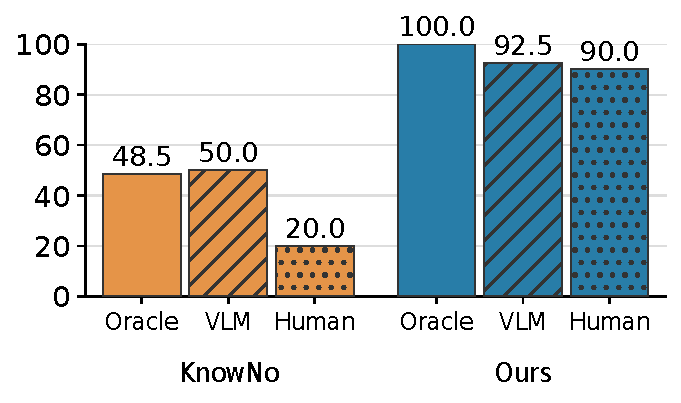
\includegraphics[width=\linewidth,height=.20\textheight,keepaspectratio]{figures/07_RESPONSE_COMPARISON/exp_response_waste_success.pdf}
% \caption{Sort Success rate (\%)}
% \label{fig:response_response_waste_success}
% \end{subfigure}
% \hfill
% \begin{subfigure}[t]{0.495\textwidth}
% \centering
% 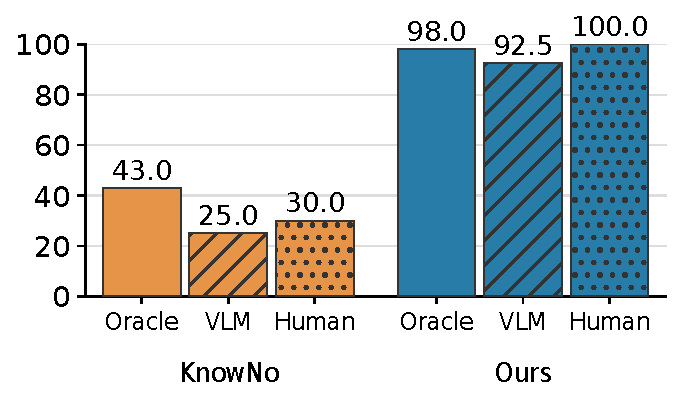
\includegraphics[width=\linewidth,height=.20\textheight,keepaspectratio]{figures/07_RESPONSE_COMPARISON/exp_response_tomato_success.pdf}
% \caption{Harvest Success rate (\%)}
% \label{fig:response_response_tomato_success}
% \end{subfigure}
% \par\medskip
% \begin{subfigure}[t]{0.495\textwidth}
% \centering
% 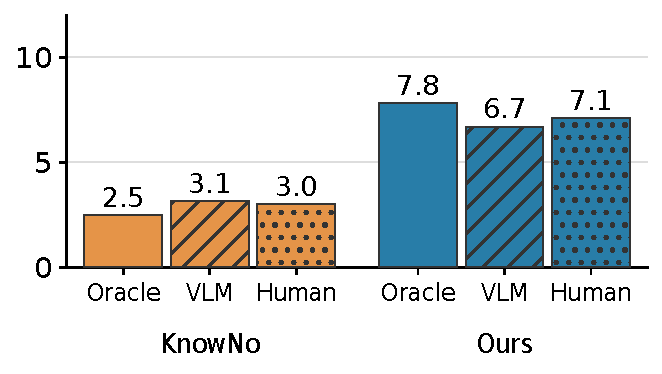
\includegraphics[width=\linewidth,height=.20\textheight,keepaspectratio]{figures/07_RESPONSE_COMPARISON/exp_response_waste_queries.pdf}
% \caption{Sort Query count}
% \label{fig:response_response_waste_queries}
% \end{subfigure}
% \hfill
% \begin{subfigure}[t]{0.495\textwidth}
% \centering
% 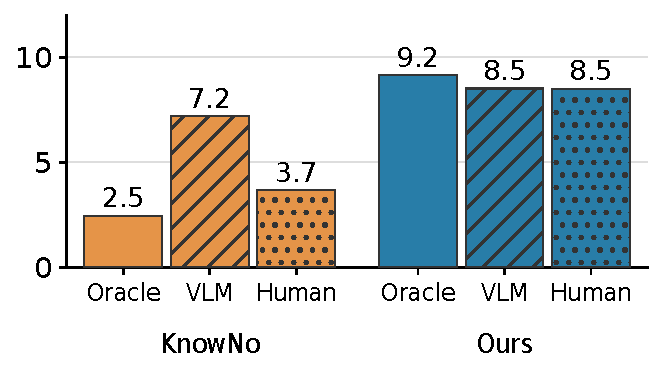
\includegraphics[width=\linewidth,height=.20\textheight,keepaspectratio]{figures/07_RESPONSE_COMPARISON/exp_response_tomato_queries.pdf}
% \caption{Harvest Query count}
% \label{fig:response_response_tomato_queries}
% \end{subfigure}
% \caption{Comparison across oracle, VLM, and human responses. Success rates are compared for Sort (a) and Harvest (b). Query counts are compared for Sort (c) and Harvest (d). Oracle trials use simulation, while VLM and human trials use physical robots.}\label{fig:response_comparison}
% \end{figure*}



% 

\subsubsection{Ablation Study}~\label{exp:when_what_random}\label{exp:policy_ablation}
% The ablation study isolates the effects of query timing and query selection on task success and query count. We compare seven configurations with oracle feedback.
The baseline comparison evaluates complete planning systems with different action planners and query policies. The ablation study examines the effects of query timing and query selection on task success and query count using seven configurations that share the POMCP action planner, with oracle feedback. For concise reference, we use \textbf{T} to label query timing variants and \textbf{S} to label query selection variants. With entropy gain selection fixed, we compare random (T1), conformal prediction (T2), and reward-based (T3) timing. With confidence timing fixed, we compare random (S1) and reward-based (S2) selection. R randomizes both query timing and query selection, while Ours combines confidence timing with entropy gain selection. Table~\ref{tab:query_strategy_matrix} summarizes these configurations. Each configuration has $200$ trials per domain. Table~\ref{tab:policy_ablation} and Fig.~\ref{fig:policy_ablation_results} present the results. Appendix~\ref{appx:ablation_configs} provides the query policy configurations.

\begin{figure}[!tp]
\centering
\captionsetup[subfigure]{font=footnotesize,skip=1pt}
\begin{minipage}[t]{0.5\columnwidth}
\vspace{0pt}
\begin{subfigure}[t]{\linewidth}
\centering
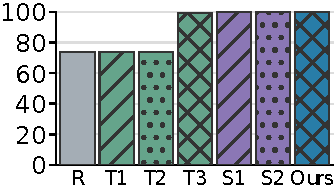
\includegraphics[width=\linewidth]{figures/08_ABLATION/exp_ablation_waste_success.pdf}
\caption{Sort Success rate (\%)}
\label{fig:ablation_ablation_waste_success}
\end{subfigure}
\par\vspace{1pt}
\begin{subfigure}[t]{\linewidth}
\centering
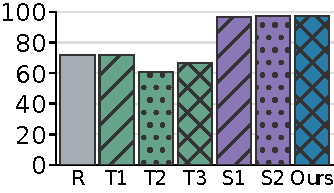
\includegraphics[width=\linewidth]{figures/08_ABLATION/exp_ablation_tomato_success.pdf}
\caption{Harvest Success rate (\%)}
\label{fig:ablation_ablation_tomato_success}
\end{subfigure}
\end{minipage}%
\begin{minipage}[t]{0.5\columnwidth}
\vspace{0pt}
\begin{subfigure}[t]{\linewidth}
\centering
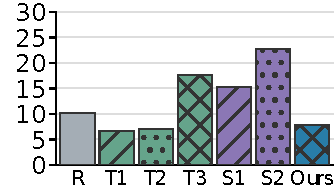
\includegraphics[width=\linewidth]{figures/08_ABLATION/exp_ablation_waste_queries.pdf}
\caption{Sort Query count}
\label{fig:ablation_ablation_waste_queries}
\end{subfigure}
\par\vspace{1pt}
\begin{subfigure}[t]{\linewidth}
\centering
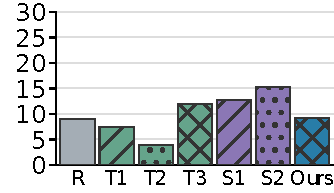
\includegraphics[width=\linewidth]{figures/08_ABLATION/exp_ablation_tomato_queries.pdf}
\caption{Harvest Query count}
\label{fig:ablation_ablation_tomato_queries}
\end{subfigure}
\end{minipage}
\caption{Results of the ablation study. (a)-(b) Confidence-based timing maintains high success rates in both domains. (c)-(d) Entropy-based selection reduces query counts compared with S1--S2. Our method achieves high task success while reducing query count.}
\label{fig:policy_ablation_results}
\end{figure}


\begin{table*}[t]
\centering
\caption{Query policy ablation. T1--T3 compare timing criteria and S1--S2 compare selection criteria. Highest success rates and lowest query counts are underlined, including ties.}
\label{tab:policy_ablation}
\label{tab:when_what_random}
\small
\setlength{\tabcolsep}{4pt}
\begin{tabular}{lllcccc}
\toprule
 & & & \multicolumn{2}{c}{Sort} & \multicolumn{2}{c}{Harvest} \\
\cmidrule(lr){4-5}\cmidrule(lr){6-7}
Condition & Timing & Selection & Success (\%) & Queries & Success (\%) & Queries \\
\midrule
R & Random & Random & 73.50 & $10.25 \pm 6.11$ & 72.00 & $9.08 \pm 3.94$ \\
T1 & Random & Entropy Gain & 73.50 & $\underline{6.65} \pm 3.29$ & 72.00 & $7.44 \pm 2.73$ \\
T2 & Conformal Prediction & Entropy Gain & 74.00 & $7.09 \pm 2.58$ & 60.50 & $\underline{3.91} \pm 1.71$ \\
T3 & Reward & Entropy Gain & 99.00 & $17.65 \pm 2.89$ & 66.50 & $12.02 \pm 2.88$ \\
S1 & Confidence & Random & \underline{100.00} & $15.21 \pm 3.53$ & 96.50 & $12.70 \pm 2.53$ \\
S2 & Confidence & Reward & \underline{100.00} & $22.79 \pm 6.26$ & 97.00 & $15.27 \pm 2.95$ \\
\textbf{Ours} & Confidence & Entropy Gain & \textbf{\underline{100.00}} & $\boldsymbol{7.83 \pm 2.16}$ & \textbf{\underline{97.50}} & $\boldsymbol{9.16 \pm 1.91}$ \\
\bottomrule
\end{tabular}
\end{table*}

The timing comparison evaluates R, T1--T3, and Ours. In Sort, R and T1 achieve $73.50\%$ success, and T2 achieves $74.00\%$. T3 achieves $99.00\%$ compared with $100.00\%$ for Ours, but requires $17.65$ queries compared with $7.83$. R, T1, and T2 use $10.25$, $6.65$, and $7.09$ queries respectively. In Harvest, R and T1 achieve $72.00\%$ success, while T2 and T3 achieve $60.50\%$ and $66.50\%$ compared with $97.50\%$ for Ours. Mean query counts are $9.08$ for R, $7.44$ for T1, $3.91$ for T2, $12.02$ for T3, and $9.16$ for Ours.

These results show that task success depends on the query trigger as well as query selection. T1 replaces random selection in R with entropy gain and reduces query count without improving success. Random timing can miss necessary verification because the trigger does not depend on current state uncertainty. T2 can also end queries after the action prediction set narrows to one candidate, even if the state facts required to execute the candidate action remain uncertain. T3 uses expected task reward to determine whether to initiate queries, then selects queries by entropy gain and repeats verification until confidence reaches $\tau$. In Sort, object category verification directly informs the correct bin choice and task reward, so repeated verification may support the high success rate of $99.00\%$. However T3 requires $125.42\%$ more queries than Ours. In Harvest, T3 uses $31.22\%$ more queries than Ours, but the success rate of T3 is $31.00$ percentage points lower. Therefore reward-based timing can request more queries overall and still fail to verify necessary state information at the appropriate time. Thus Ours uses current state confidence as the query trigger and achieves the highest success in both domains with fewer queries than reward-based timing.

With confidence-based query timing fixed, different query selection strategies maintain high success rates but require different numbers of queries. The query selection comparison evaluates R, S1, S2, and Ours. R achieves $73.50\%$ success in Sort and $72.00\%$ in Harvest with $10.25$ queries in Sort and $9.08$ in Harvest. S1 retains random selection but uses confidence timing, and success increases to $100.00\%$ and $96.50\%$ respectively. With confidence timing fixed, S1, S2, and Ours all achieve $100.00\%$ success in Sort. Mean query counts are $15.21$ for S1, $22.79$ for S2, and $7.83$ for Ours. In Harvest, S1 and S2 achieve $96.50\%$ and $97.00\%$ success, respectively, compared with $97.50\%$ for Ours. Mean query counts are $12.70$ for S1, $15.27$ for S2, and $9.16$ for Ours.

Confidence timing maintains $100.00\%$ success in Sort and at least $96.50\%$ in Harvest across all three query selection strategies. Under confidence timing, query selection primarily affects the number of queries needed to reach the required confidence. Random selection does not prioritize facts by their expected reduction in state uncertainty. Reward-based selection evaluates expected task reward without directly measuring the information provided by a query response. Entropy gain selects facts according to the expected reduction in state uncertainty, so the selection criterion matches the confidence requirement that ends a query episode. Relative to S1 and S2, Ours reduces query count by $48.52\%$ and $65.64\%$ in Sort and by $27.87\%$ and $40.01\%$ in Harvest. Thus our query selection method reduces the number of queries required under confidence timing without reducing task success.

These results support the main contribution of our method through the distinct roles of query timing and query selection. Query timing determines whether the robot requests additional information before it executes actions under state uncertainty. Confidence timing achieves high success with random, reward-based, and entropy gain selection, while entropy gain under random timing reduces query count without improving success over R. Once confidence timing establishes a high success level, entropy gain reduces the number of queries needed to reach the required confidence. Therefore our method combines a timing criterion that supports task success with a selection criterion that reduces query count at that success level.

\subsubsection{Threshold Experiments}~\label{exp:sys_threshold}
After the ablation comparison, we examine how the confidence threshold controls task success and query count. We vary $\tau$ from $0.0$ to $1.0$ in increments of $0.1$ with entropy gain selection fixed and correct oracle responses in simulation. Each threshold has $200$ trials per domain. At $\tau=0.8$, we reuse the Ours trials reported in Tables~\ref{tab:baseline_results} and~\ref{tab:policy_ablation}. Fig.~\ref{fig:threshold_results} presents the results.

\begin{figure}[!tp]
\centering
\begin{subfigure}[t]{0.5\columnwidth}
\centering
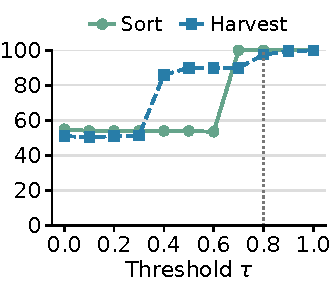
\includegraphics[width=\linewidth]{figures/09_THRESHOLD/exp_threshold_success.pdf}
\caption{Task success}
\label{fig:threshold_success}
\end{subfigure}%
\begin{subfigure}[t]{0.5\columnwidth}
\centering
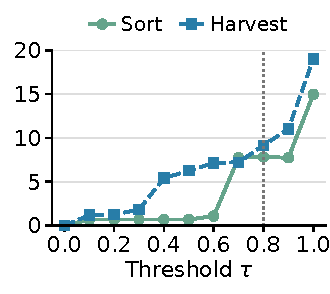
\includegraphics[width=\linewidth]{figures/09_THRESHOLD/exp_threshold_queries.pdf}
\caption{Mean query count}
\label{fig:threshold_queries}
\end{subfigure}
\caption{Effect of the confidence threshold $\tau$ on task success and query count. (a) Task success reaches $100.00\%$ at $\tau=0.7$ in Sort and $100.00\%$ at $\tau=1.0$ in Harvest. (b) Mean query count increases sharply at $\tau=1.0$ in both domains. Relative to the default $\tau=0.8$ (dotted line), $\tau=1.0$ roughly doubles query count while success remains unchanged in Sort and increases by $2.50\%p$ in Harvest.}
\label{fig:threshold_results}
\end{figure}

Fig.~\ref{fig:threshold_results} shows different responses to the confidence threshold across the two domains. In Sort, success increases from $53.50\%$ at $\tau=0.6$ to $100.00\%$ at $\tau=0.7$ and remains unchanged at higher thresholds. Mean query counts range from $7.74$ to $7.83$ over $\tau=0.7$--$0.9$ and increase to $14.97$ at $\tau=1.0$. In Harvest, success rises from $51.50\%$ at $\tau=0.3$ to $86.00\%$ at $\tau=0.4$ and remains $90.00\%$ over $\tau=0.5$--$0.7$. Further increases in the threshold yield $97.50\%$ success at $\tau=0.8$, $99.50\%$ at $\tau=0.9$, and $100.00\%$ at $\tau=1.0$. Mean query count increases from $5.41$ at $\tau=0.4$ to $9.16$ at $\tau=0.8$ and $19.00$ at $\tau=1.0$.

System-initiated querying improves task success under the same POMCP action planner. Without queries ($\tau=0.0$), Ours achieves $55.00\%$ success in Sort and $51.00\%$ in Harvest. Both rates exceed those of KnowNo and IntroPlan with oracle feedback. At $\tau=0.8$, success increases by $45.00$ and $46.50$ percentage points, respectively. Successful trials require an average of $7.83$ queries in Sort and $9.16$ in Harvest.

Additional queries provide limited gains once task success approaches its maximum. Raising $\tau$ from $0.8$ to $1.0$ increases mean query count by $91.19\%$ in Sort and $107.42\%$ in Harvest, but success increases by $0.00$ and $2.50$ percentage points, respectively. In Harvest, the final increase from $\tau=0.9$ to $1.0$ alone adds $7.98$ queries for only $0.50$ percentage points of additional success. We use $\tau=0.8$ as a common threshold to balance task success and query count across both domains.


\subsubsection{Interviews}\label{exp:interviews}
% We interview all five participants after they experience both methods in Sort and Harvest. Participants describe Ours as asking them to verify the current state and KnowNo as asking them to choose the next action. In KnowNo, P1 expects some action choices to include preceding steps, P2 is unsure whether all candidate actions are currently executable, and P4 considers which steps have to occur first. These reports suggest that answering action-selection queries requires participants to interpret both what each action executes and which preconditions have to be satisfied. Differences in these interpretations help explain the action-selection failures analyzed earlier.
We interview all five participants after they use Ours and KnowNo in both domains. P1 and P2 describe Ours as more reliable than KnowNo for completing the evaluated tasks. P1 considers errors less likely with Ours. P2 expects Ours to complete the task after receiving state confirmations, whereas KnowNo sometimes fails after P2 selects actions that appear executable from the camera view.

% Four participants (P1--P4) prefer Ours for the evaluated tasks. P1 and P2 describe smoother task progress and greater perceived efficiency, while P3 and P4 emphasize convenience and less deliberation about subsequent actions. P3 finds frequent questions bothersome despite preferring Ours, and P5 prefers KnowNo because directly selecting or entering a command feels more convenient than repeated confirmations. Interview results indicate that preferences reflect both the judgments required to answer queries and the frequency and form of participation.
Selecting the correct action requires participants to interpret both the scope of each action and the preceding steps needed for execution. P1 expects KnowNo to perform picking as part of a subsequent action, such as checking tomato quality. P3 recalls a failure after selecting a quality check before picking, and P4 attributes a tomato-task failure to skipping a required stage. The reported failures match the failure analysis, which identifies KnowNo failures following selections that omit required preceding actions. Ours asks participants to verify state facts and leaves action selection and sequencing to the planner. Participants therefore do not need to determine whether an action choice includes the necessary preceding steps. This division of responsibilities helps explain the higher task success rate of Ours in the human evaluation.


\subsubsection{Discussion and Limitation}\label{exp:discussion}
We find that query timing primarily affects task success, while query selection primarily affects the number of queries required. The ablation study shows that confidence-based timing maintains high success across selection strategies, while entropy-based selection reduces query counts when timing is fixed. Our method combines confidence-based timing with entropy-based selection to balance task success and query efficiency. Across Sort and Harvest, our method achieves the highest task success among the evaluated methods in simulation and with VLM and human feedback on physical robots.



Efficient query selection reduces the number of queries needed to reach a given confidence level. The confidence threshold controls the trade-off between accepting uncertainty and requesting further verification. If $\tau<1$, the robot may commit to a state while alternative states retain belief weight. Accepting uncertainty can reduce query counts, but an incorrect state estimate may affect subsequent actions. If $\tau=1$, the robot resumes execution only after belief entropy reaches zero. Our threshold experiments show that increasing the number of queries does not necessarily improve task success rates. The benefit of additional queries depends on whether the remaining uncertainty affects task success. The two domains also require different confidence levels to achieve a high task success rate. 



A limitation of our method is that the belief update does not account for errors in responses from external agents. State hypotheses inconsistent with answers are removed regardless of response reliability. Incorrect feedback can therefore exclude the true state from the belief and leave the robot confident in an incorrect state. The failures involving incorrect VLM and human responses illustrate the practical impact of feedback errors. Raising the confidence threshold cannot ensure a correct state estimate, because confidence is computed over the remaining hypotheses. Incorporating response reliability into the belief update could preserve plausible alternatives by adjusting hypothesis weights instead of removing inconsistent hypotheses outright.

% % Keep the experimental figures and tables before the conclusion.
% \clearpage

\section{Conclusion and Future Work}
We presented a method that uses state uncertainty to determine when and what to query during robot task planning. Belief confidence determines query timing, and expected entropy reduction guides the selection of state facts. Experiments in Sort and Harvest show that query timing supports task success, while query selection reduces the number of required queries. Future work will incorporate response reliability into belief updates to improve robustness to incorrect answers from external agents.

\bmhead{Acknowledgements}
This research was supported in part by the National Research Foundation of Korea (NRF) grant funded by the Korea government (MSIT)(No. RS-2024-00461583) and the National Research Foundation of Korea (NRF) grant funded by the Korea government (MSIT) (No. RS-2024-00411007).

\bmhead{Ethics approval and consent}
This study was approved by the Institutional Review Board of Sogang University (Approval No. SGUIRB-A-2501-04-2). The study was conducted in accordance with the ethical standards of the institution. Informed consent was obtained from all participants before participation.

% \bibliography{ref}
\bibliography{ref}

\begin{appendices}
\onecolumn
\section{Experimental Parameters}\label{appx:settings}
\subsection{Shared Settings}\label{appx:planner_params}
Table~\ref{tab:app_planner_params} lists the shared settings. Oracle trials use $200$ trials per domain and condition. Physical evaluations use $40$ VLM trials and $10$ human trials per method and domain.

\begin{table}[!htbp]
\centering
\caption{Shared planner and evaluation parameters.}
\label{tab:app_planner_params}
\small
\begin{tabular*}{\textwidth}{@{\extracolsep{\fill}}lclc@{}}
\toprule
Parameter & Value & Parameter & Value \\
\midrule
POMCP simulations per step & $100$ & Maximum simulation depth & $20$ \\
Default discount factor $\gamma$ & $0.2$ & UCB exploration constant $c$ & $1.0$ \\
Confidence threshold $\tau$ & $0.8$ & Discount cutoff $\epsilon$ & $0.005$ \\
\bottomrule
\end{tabular*}
\end{table}
With $\gamma=0.2$ and $\epsilon=0.005$, the discount cutoff stops simulations at depth $4$. In the oracle experiments, we allow at most $20$ physical actions per trial. For POMCP-Q, we also allow at most $30$ queries per trial.

\subsection{Reward Settings}\label{appx:rewards}
Table~\ref{tab:app_rewards} lists the domain rewards used for action planning and reward-based query evaluation. Goal and action rewards are additive. Other applicable physical actions have zero reward.

\begin{table}[!htbp]
\centering
\caption{Task rewards and penalties.}
\label{tab:app_rewards}
\small
\begin{tabularx}{\textwidth}{@{}lXr@{}}
\toprule
Domain & Outcome or action & Reward \\
\midrule
Sort & Place an object in the correct bin & $+5$ \\
 & Reach the task goal & $+10$ \\
 & Third and subsequent consecutive detection actions & $-10$ \\
\addlinespace[3pt]
Harvest & Place a fresh tomato or discard a rotten tomato & $+10$ \\
 & Second and subsequent consecutive detections at the same stem & $-5$ \\
 & Second and subsequent consecutive scans of the same tomato & $-5$ \\
 & Second and subsequent consecutive navigation actions & $-5$ \\
\bottomrule
\end{tabularx}
\end{table}

POMCP-Q and the reward evaluators in T3 and S2 use the same domain rewards. Their value models assign zero immediate reward to each query and a penalty of $-10$ to an inapplicable physical action.

\subsection{Baseline Parameters}\label{appx:baseline_configs}
Table~\ref{tab:app_baseline_params} gives domain-specific settings. KnowNo and IntroPlan use GPT-4o with an action generation temperature of $0.3$ and a score temperature of $5.0$. The calibration thresholds $\hat{q}$ for KnowNo and IntroPlan target $95\%$ prediction-set coverage. Under the exchangeability assumption, conformal prediction guarantees that the prediction set contains at least one correct action with probability at least $0.95$~\citep{ren2023robots}. 

POMCP-Q uses $100$ simulations per decision, zero query cost, a failure penalty of $10$, and assumed response accuracy $1.0$. The discount factor $\gamma$ and other POMCP-Q settings are selected separately for each domain based on the highest task success rate among the evaluated configurations. A dash denotes an inapplicable setting.

\begin{table}[!htbp]
\centering
\caption{Baseline parameters for Sort and Harvest.}
\label{tab:app_baseline_params}
\footnotesize
\setlength{\tabcolsep}{2pt}
\renewcommand{\arraystretch}{1.05}
\setlength{\extrarowheight}{0pt}
\begin{tabular*}{\textwidth}{@{\extracolsep{\fill}}llcccc@{}}
\toprule
Domain & Parameter & \textbf{Ours} & KnowNo & IntroPlan & POMCP-Q \\
\midrule
\multirow{3}{*}{Sort} & Calibration threshold $\hat{q}$ (oracle) & --- & $0.845165$ & $0.980493$ & --- \\
 & Action generation temperature (oracle) & --- & $0.3$ & $0.3$ & --- \\
 & Discount factor $\gamma$ & $0.2$ & --- & --- & $0.9$ \\
\addlinespace[3pt]
\multirow{3}{*}{Harvest} & Calibration threshold $\hat{q}$ (oracle) & --- & $0.901119$ & $0.985552$ & --- \\
 & Action generation temperature (oracle) & --- & $0.3$ & $0.3$ & --- \\
 & Discount factor $\gamma$ & $0.2$ & --- & --- & $0.5$ \\
\bottomrule
\end{tabular*}
\end{table}

\subsection{Ablation Parameters}\label{appx:ablation_configs}
Table~\ref{tab:app_ablation_params} specifies query timing and selection. CP denotes conformal prediction, and Entropy denotes expected entropy reduction. All configurations use $100$ POMCP simulations per step and $\tau=0.8$. T3 and S2 use zero query cost, a failure penalty of $10$, and assumed response accuracy $1.0$. For T3 and S2, we select the discount factor $\gamma$ separately for each domain based on the highest task success rate among the evaluated configurations.

\begin{table}[!htbp]
\centering
\caption{Ablation parameters for Sort and Harvest.}
\label{tab:app_ablation_params}
\footnotesize
\setlength{\tabcolsep}{2pt}
\renewcommand{\arraystretch}{1.05}
\setlength{\extrarowheight}{0pt}
\begin{tabular*}{\textwidth}{@{\extracolsep{\fill}}llccccccc@{}}
\toprule
Domain & Parameter & R & T1 & T2 & T3 & S1 & S2 & \textbf{Ours} \\
\midrule
\multirow{7}{*}{Sort} & Query timing & Random & Random & CP & Reward & Confidence & Confidence & Confidence \\
 & Query selection & Random & Entropy & Entropy & Entropy & Random & Reward & Entropy \\
 & Random trigger probability & $0.4$ & $0.4$ & --- & --- & --- & --- & --- \\
 & Discount factor $\gamma$ & $0.2$ & $0.2$ & $0.2$ & $0.9$ & $0.2$ & $0.9$ & $0.2$ \\
 & Calibration threshold $\hat{q}$ & --- & --- & $0.8704$ & --- & --- & --- & --- \\
 & Candidate score temperature & --- & --- & $5.0$ & --- & --- & --- & --- \\
 & Query evaluation simulations & --- & --- & --- & $\geq 100$ & --- & $\geq 100$ & --- \\
\addlinespace[3pt]
\multirow{7}{*}{Harvest} & Query timing & Random & Random & CP & Reward & Confidence & Confidence & Confidence \\
 & Query selection & Random & Entropy & Entropy & Entropy & Random & Reward & Entropy \\
 & Random trigger probability & $0.4$ & $0.4$ & --- & --- & --- & --- & --- \\
 & Discount factor $\gamma$ & $0.2$ & $0.2$ & $0.2$ & $0.5$ & $0.2$ & $0.5$ & $0.2$ \\
 & Calibration threshold $\hat{q}$ & --- & --- & $0.8404$ & --- & --- & --- & --- \\
 & Candidate score temperature & --- & --- & $5.0$ & --- & --- & --- & --- \\
 & Query evaluation simulations & --- & --- & --- & $\geq 100$ & --- & $\geq 100$ & --- \\
\bottomrule
\end{tabular*}
\end{table}

T2 starts and continues verification while the conformal prediction set contains multiple actions. T3 starts verification when the highest query value exceeds the highest physical action value. S2 selects the highest-value fact without comparing its value with physical actions. After a trigger, all configurations except T2 continue verification until confidence reaches $\tau$ or no differentiating fact remains. Four unparseable T2 outputs count as failures.

\subsection{Trial Reuse and Reporting}\label{appx:oracle_reference}\label{appx:randomization}\label{appx:metric_details}
The same $200$ \textbf{Ours} trials per domain are reused for the baseline, ablation, and threshold comparisons at $\tau=0.8$. Other thresholds use separate batches. Oracle conditions share seeds for each initial configuration and repetition, although policies can consume random numbers differently.

Success uses all trials, and other trial-level metrics use successful-trial means and sample standard deviations. Planning time is cumulative recorded search time, including candidate generation and scoring for KnowNo and IntroPlan. Oracle total time equals planning time. Human interaction time per query pools interaction time and query count across successful and failed trials.

\newtcolorbox{vlmpromptbox}[1]{
    enhanced,
    breakable,
    sharp corners,
    colback=white,
    colframe=black,
    colbacktitle=gray!10,
    coltitle=black,
    fonttitle=\bfseries,
    fontupper=\small,
    boxrule=0.4pt,
    left=3mm,
    right=3mm,
    top=2mm,
    bottom=2mm,
    before skip=10pt,
    after skip=10pt,
    title={#1},
    title after break={}
}

\section{VLM Prompts}\label{appx:vlm_prompts}

Both domains use \texttt{nvidia/Gemma-4-31B-IT-NVFP4} with a sampling temperature of $0.3$. Each request includes two current RGB camera images, the current robot action, and the domain action model. Ours supplies a Korean state-verification question and criteria for the queried predicate. KnowNo supplies candidate actions, response tokens, and criteria for action selection. Harvest also supplies fixed object identifiers and stem assignments. The boxes summarize the prompt instructions in English; supplementary configuration files preserve the original English and Korean text.

\begin{vlmpromptbox}{Shared Request Instructions}
State verification requires Yes or No on the first line and a concise reason on the second. The client converts the answer to a Boolean value for the belief update. Action selection requires a candidate token followed by a concise Korean reason. The VLM checks object identity, robot state, and action preconditions from the images. Attempted actions do not establish successful execution or satisfied preconditions. If no candidate meets the execution conditions, the VLM selects the option for manual action entry. The client checks that the returned token belongs to the candidate set.
\end{vlmpromptbox}

\begin{vlmpromptbox}{Sort Domain Instructions}
The VLM identifies the queried object by its number and checks visibility, material, and shape. Occlusion does not establish absence, and color or a candidate bin name alone does not establish category. Gripper and bin contents provide evidence for holding and placement facts. Detection must precede picking, including for newly exposed objects. Picking requires an empty gripper; placement requires holding the object and matching its category to the bin. Visible objects and bounding boxes do not establish completed detection. Completion requires an empty worktable, correctly sorted objects, and an empty gripper.
\end{vlmpromptbox}

\begin{vlmpromptbox}{Harvest Domain Instructions}
The VLM uses fixed tomato identifiers and ArUco markers to determine location. Dominant red or green color determines ripeness. A large beige rotten area indicates rot; minor scratches, reflections, and discoloration do not. The VLM inspects the held tomato using both camera views and checks gripper and basket contents directly. Navigation and detection require an empty gripper. Picking requires completed detection and a ripe tomato at the current stem. Scanning follows picking and determines whether the tomato should be placed or discarded. Visible tomatoes and attempted actions do not establish completed detection or scanning. Completion requires no remaining ripe tomatoes to process and an empty gripper.
\end{vlmpromptbox}

\section{Human Evaluation and Interviews}\label{appx:user}
\subsection{Instructions and Trial Order}\label{appx:user_scenarios}\label{appx:user_assignment}
Participants receive task goals, object categories, and available actions, then answer queries through a tablet displaying camera views (Fig.~\ref{fig:app_human_tablet}). Ours requests Boolean state confirmations, potentially several per episode. KnowNo requests one action choice per trigger and permits manual entry. Each participant completes two trials per method and domain.

Let A denote Ours and B denote KnowNo. P1 and P5 complete Sort before Harvest with method order AABB. P2 completes the domains in reverse order with ABAB. P3 follows Sort then Harvest with BBAA, and P4 follows the reverse domain order with BABA. Each method sequence applies to both domains.

\begin{figure}[t]
\centering
\captionsetup[subfigure]{font=small,skip=2pt}
\begin{subfigure}[t]{0.485\linewidth}
\centering
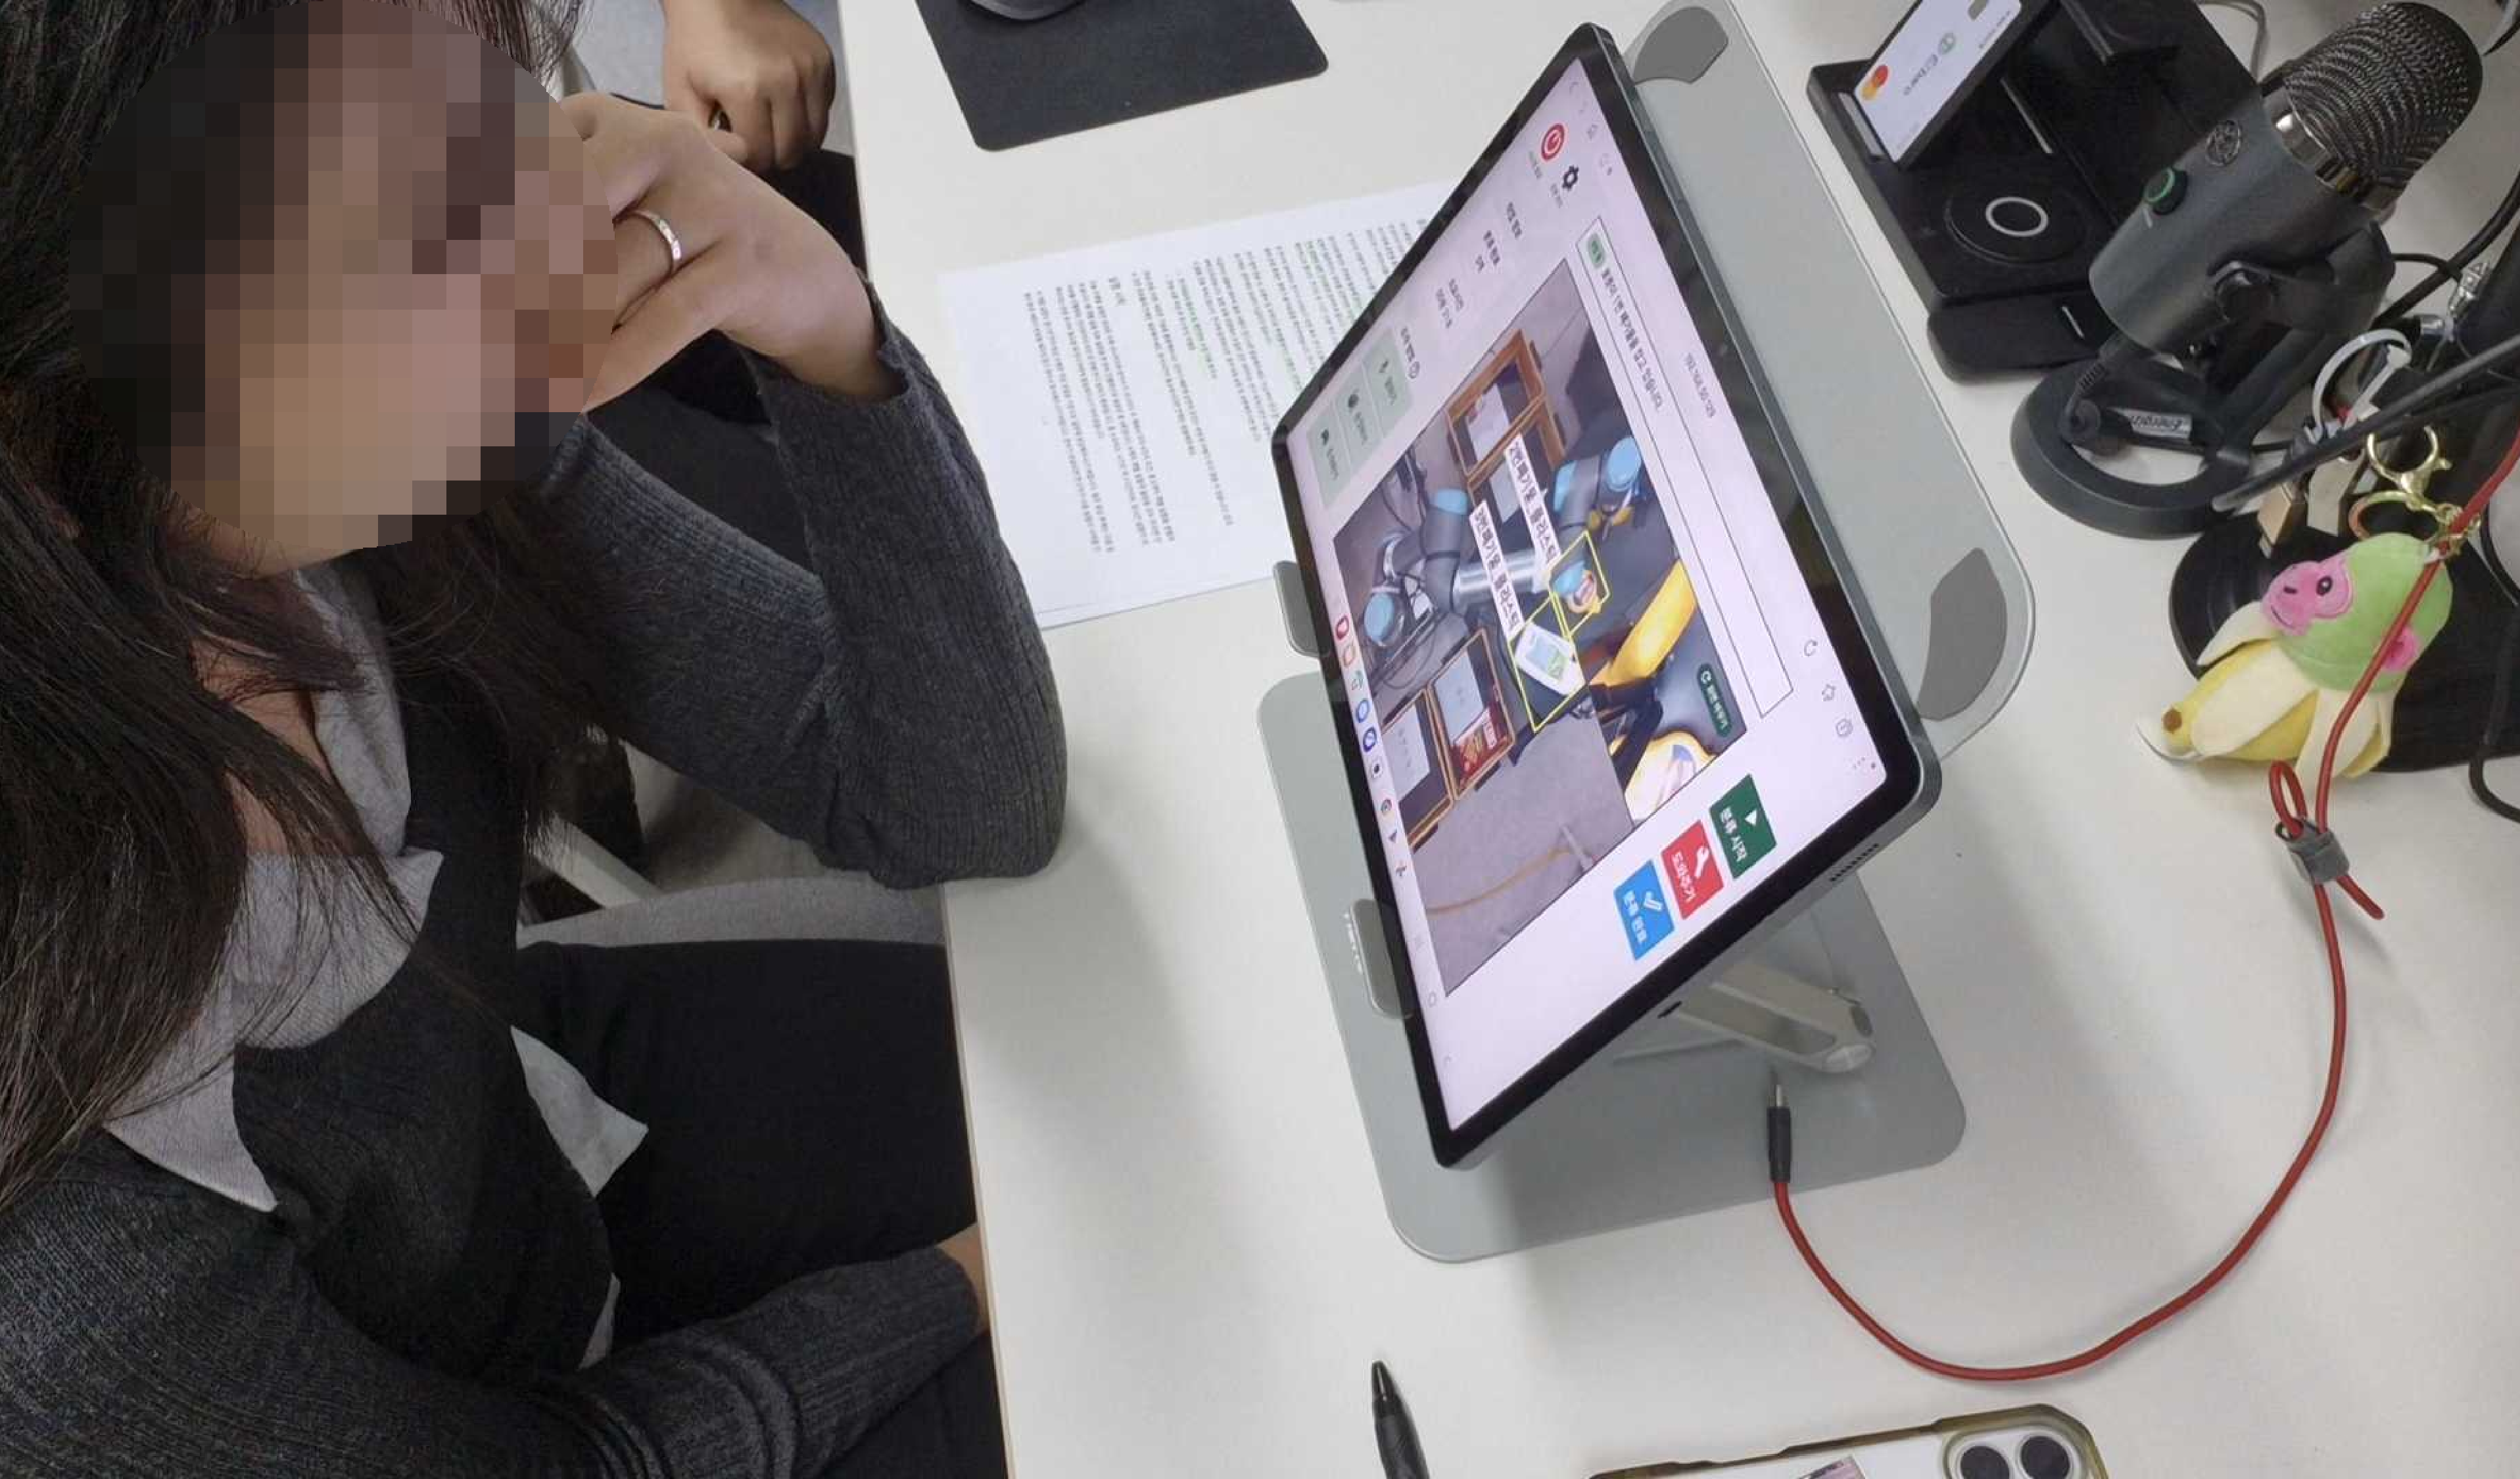
\includegraphics[width=\linewidth]{figures/10_APPX/p3_test.pdf}
\caption{P3, Sort}
\label{fig:app_human_sort}
\end{subfigure}\hfill%
\begin{subfigure}[t]{0.485\linewidth}
\centering
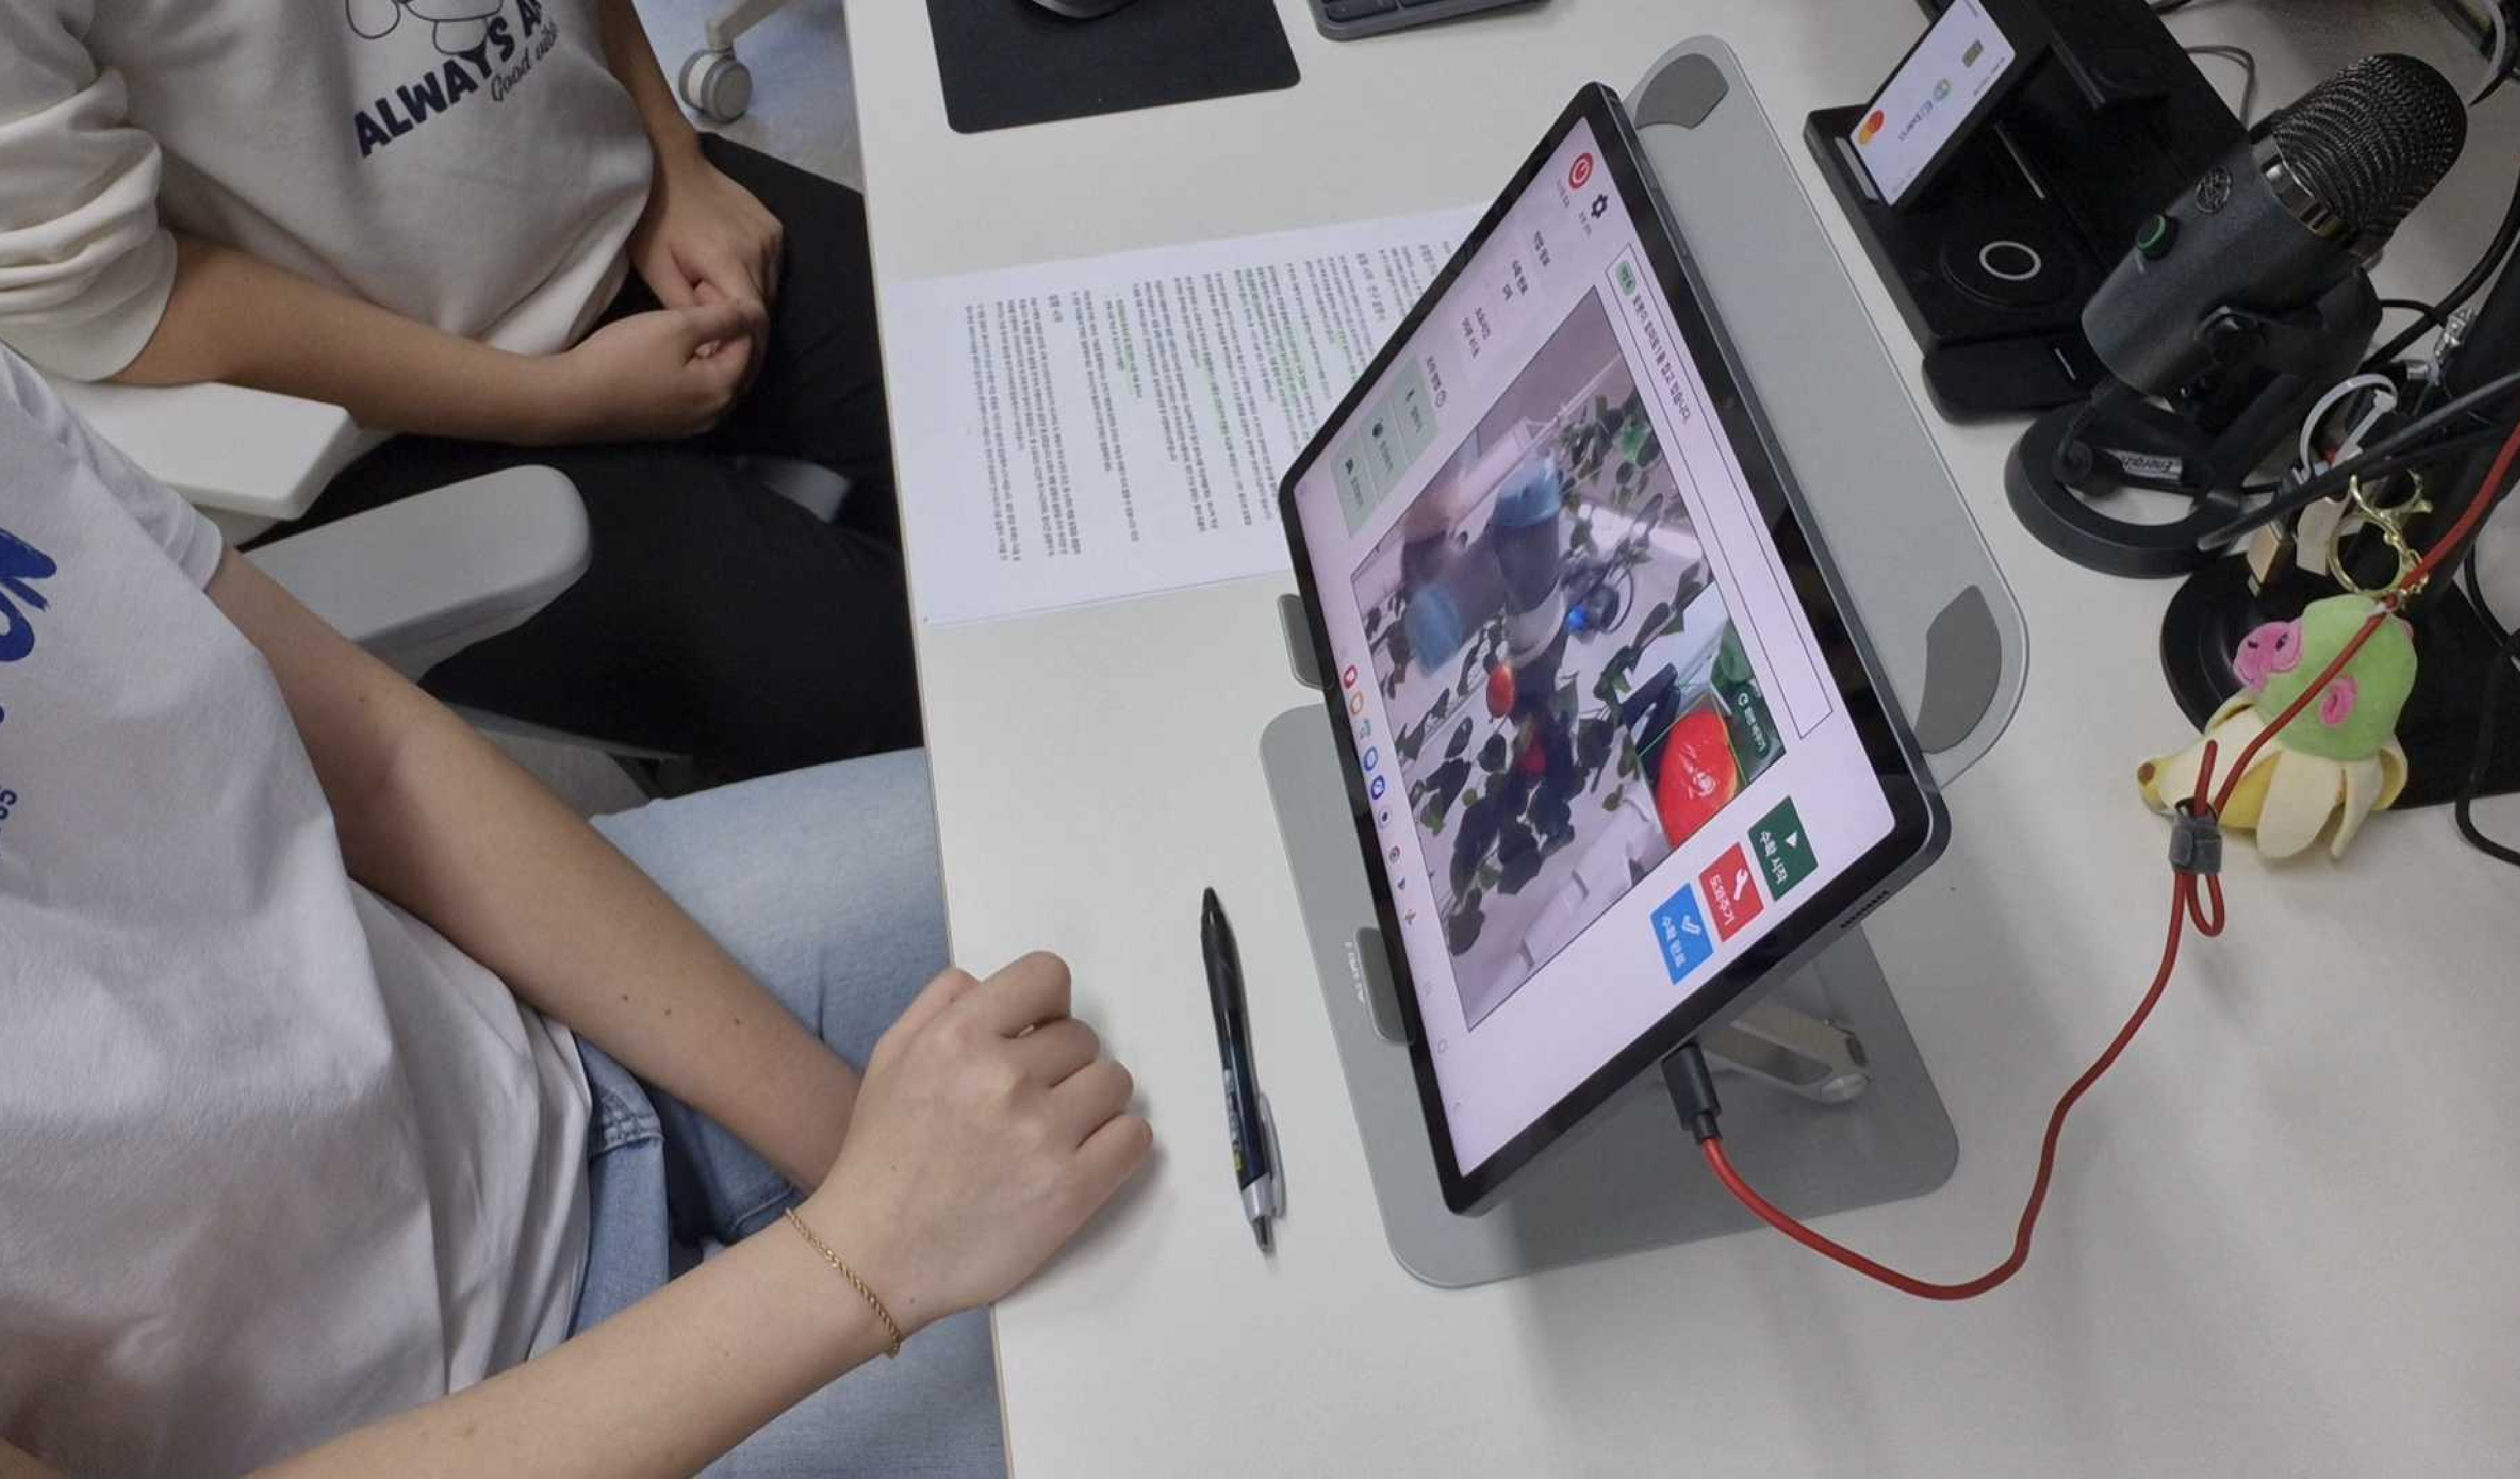
\includegraphics[width=\linewidth]{figures/10_APPX/p2_test.pdf}
\caption{P2, Harvest}
\label{fig:app_human_harvest}
\end{subfigure}
\caption{Human evaluation using the tablet interface. (a)-(b) Participants view robot camera feeds and answer queries in Sort and Harvest, respectively.}
\label{fig:app_human_tablet}
\end{figure}

\subsection{Interview Summary}\label{appx:user_interviews}
Table~\ref{tab:app_interview_summary} summarizes the five interviews discussed in Sec.~\ref{exp:interviews}.
% Excerpts are translated from Korean with speech fillers omitted. Bracketed method names replace interview labels A/B.

\begin{table}[!htbp]
\centering
\caption{Interview excerpts on baseline comparison with human response.}
\label{tab:app_interview_summary}
\small
\setlength{\tabcolsep}{5pt}
\renewcommand{\arraystretch}{1.12}
\begin{tabularx}{\textwidth}{@{}l>{\hsize=1.25\hsize\linewidth=\hsize\raggedright\arraybackslash}X>{\hsize=.75\hsize\linewidth=\hsize\raggedright\arraybackslash}X@{}}
\toprule
Participant & Interview excerpts & Interpretation \\
\midrule
% Sources: 08_Delete_Me/00_real_human/p001/p001_v2.txt, participant turns at lines 286--287 and 241--242.
P1 & ``I think errors are much less likely with [Ours].''\par For KnowNo: ``I expected it to pick the object and check its quality.'' & Links perceived reliability to fewer errors and identifies an expectation that a selected action includes preceding steps. \\
\addlinespace
% Source: 08_Delete_Me/00_real_human/p002/p002_v1.txt, participant turn at lines 476--477.
P2 & ``With [Ours], I assume the task will be completed unless I give an incorrect answer. With [KnowNo], the choices looked executable on the screen, but some did not work after I selected them.'' & Connects expected task completion with state confirmation and reports failed execution despite apparently feasible choices. \\
\addlinespace
% Source: 08_Delete_Me/00_real_human/p003/p003_v1.txt, participant turn at lines 148--149.
P3 & ``I chose the quality check because I was focused on the goal, but perhaps because I selected it before picking, it showed a failure.'' & Matches the Harvest failures involving actions selected before their preconditions are satisfied. \\
\addlinespace
% Sources: 08_Delete_Me/00_real_human/p004/p004_v1.txt, participant turns at lines 59--61 and 246--247.
P4 & For KnowNo: ``Looking back, I think I skipped a stage because I was impatient, and that seems to be why it failed.''\par For Ours: ``I only assess the state, and the robot handles most of the actions.'' & Links skipped stages to failure and describes leaving subsequent actions to the robot, supporting the division of responsibilities discussed in the main text. \\
\addlinespace
% Source: 08_Delete_Me/00_real_human/p005/p005_v1.txt, participant turn describing fact confirmation and action commands.
P5 & ``One robot asked whether something was correct; the other asked me to specify the next action.'' & Distinguishes fact verification from action decisions, consistent with the roles assigned to participants in the two methods. \\
\bottomrule
\end{tabularx}
\end{table}

\end{appendices}

\end{document}
